\documentclass[11pt,]{article}
\usepackage{lmodern}
\usepackage{amssymb,amsmath}
\usepackage{ifxetex,ifluatex}
\usepackage{fixltx2e} % provides \textsubscript
\ifnum 0\ifxetex 1\fi\ifluatex 1\fi=0 % if pdftex
  \usepackage[T1]{fontenc}
  \usepackage[utf8]{inputenc}
\else % if luatex or xelatex
  \ifxetex
    \usepackage{mathspec}
  \else
    \usepackage{fontspec}
  \fi
  \defaultfontfeatures{Ligatures=TeX,Scale=MatchLowercase}
\fi
% use upquote if available, for straight quotes in verbatim environments
\IfFileExists{upquote.sty}{\usepackage{upquote}}{}
% use microtype if available
\IfFileExists{microtype.sty}{%
\usepackage{microtype}
\UseMicrotypeSet[protrusion]{basicmath} % disable protrusion for tt fonts
}{}
\usepackage[margin=0.79in]{geometry}
\usepackage{hyperref}
\hypersetup{unicode=true,
            pdftitle={A Model for Energy-Saving in an IoT Smarthome accounting for End-User Convenience},
            pdfauthor={Alistair Francis Bowman Grevis-James},
            pdfborder={0 0 0},
            breaklinks=true}
\urlstyle{same}  % don't use monospace font for urls
\usepackage{graphicx,grffile}
\makeatletter
\def\maxwidth{\ifdim\Gin@nat@width>\linewidth\linewidth\else\Gin@nat@width\fi}
\def\maxheight{\ifdim\Gin@nat@height>\textheight\textheight\else\Gin@nat@height\fi}
\makeatother
% Scale images if necessary, so that they will not overflow the page
% margins by default, and it is still possible to overwrite the defaults
% using explicit options in \includegraphics[width, height, ...]{}
\setkeys{Gin}{width=\maxwidth,height=\maxheight,keepaspectratio}
\IfFileExists{parskip.sty}{%
\usepackage{parskip}
}{% else
\setlength{\parindent}{0pt}
\setlength{\parskip}{6pt plus 2pt minus 1pt}
}
\setlength{\emergencystretch}{3em}  % prevent overfull lines
\providecommand{\tightlist}{%
  \setlength{\itemsep}{0pt}\setlength{\parskip}{0pt}}
\setcounter{secnumdepth}{5}
% Redefines (sub)paragraphs to behave more like sections
\ifx\paragraph\undefined\else
\let\oldparagraph\paragraph
\renewcommand{\paragraph}[1]{\oldparagraph{#1}\mbox{}}
\fi
\ifx\subparagraph\undefined\else
\let\oldsubparagraph\subparagraph
\renewcommand{\subparagraph}[1]{\oldsubparagraph{#1}\mbox{}}
\fi

%%% Use protect on footnotes to avoid problems with footnotes in titles
\let\rmarkdownfootnote\footnote%
\def\footnote{\protect\rmarkdownfootnote}

%%% Change title format to be more compact
\usepackage{titling}

% Create subtitle command for use in maketitle
\providecommand{\subtitle}[1]{
  \posttitle{
    \begin{center}\large#1\end{center}
    }
}

\setlength{\droptitle}{-2em}

  \title{A Model for Energy-Saving in an IoT Smarthome accounting for End-User
Convenience}
    \pretitle{\vspace{\droptitle}\centering\huge}
  \posttitle{\par}
    \author{Alistair Francis Bowman Grevis-James}
    \preauthor{\centering\large\emph}
  \postauthor{\par}
      \predate{\centering\large\emph}
  \postdate{\par}
    \date{November 2019}

\usepackage{booktabs}
\usepackage{longtable}
\usepackage{array}
\usepackage{multirow}
\usepackage[table]{xcolor}
\usepackage{wrapfig}
\usepackage{float}
\usepackage{colortbl}
\usepackage{pdflscape}
\usepackage{tabu}
\usepackage{threeparttable}
\usepackage{threeparttablex}
\usepackage[normalem]{ulem}
\usepackage{makecell}

\usepackage[ruled,vlined,linesnumbered]{algorithm2e} \SetAlFnt{\tiny} \SetAlCapNameFnt{\small} \usepackage{booktabs} \usepackage{longtable} \usepackage{array} \usepackage{multirow} \usepackage[table]{xcolor} \usepackage{wrapfig} \usepackage{float} \floatplacement{figure}{H} \usepackage{caption, setspace} \captionsetup[figure]{font={stretch=1,scriptsize}} \captionsetup[figure]{skip=2pt} \captionsetup[table]{font={stretch=1,scriptsize}} \captionsetup[table]{skip=2pt}

\begin{document}
\maketitle

{
\setcounter{tocdepth}{3}
\tableofcontents
}
\pagebreak

Test for in \ref{fig:fig1} we see XYZ

\hypertarget{introduction}{%
\section{Introduction}\label{introduction}}

\begin{itemize}
\tightlist
\item
  Using only accuracy as a metric, the original, top 5 and electrical
  only were compared.
\end{itemize}

A decision tree classifier

The reported averages include macro average (averaging the unweighted
mean per label), weighted average (averaging the support-weighted mean
per label)
\url{https://scikit-learn.org/stable/modules/generated/sklearn.metrics.classification_report.html}

The last line gives a weighted average of precision, recall and f1-score
where the weights are the support values. so for precision the avg is
(0.50\emph{1 + 0.0}1 + 1.0*3)/5 = 0.70. The total is just for total
support which is 5 here.

Compute the F1 score, also known as balanced F-score or F-measure

The F1 score can be interpreted as a weighted average of the precision
and recall, where an F1 score reaches its best value at 1 and worst
score at 0. The relative contribution of precision and recall to the F1
score are equal. The formula for the F1 score is:

F1 = 2 * (precision * recall) / (precision + recall)
\url{https://scikit-learn.org/stable/modules/generated/sklearn.metrics.f1_score.html}

\pagebreak

\hypertarget{bedroom-lightswitch}{%
\subsubsection{Bedroom Lightswitch}\label{bedroom-lightswitch}}

\begin{itemize}
\tightlist
\item
  Confusion matrix
\item
  KPIs
\end{itemize}

best params: \{`criterion': `entropy', `max\_depth': 4\} best score:
0.9795956924239562 best features: {[}`bathroom\_lightswitch'
`kitchen\_cabinet' `kitchen\_dishwasher' `kitchen\_laundrydryer'
`livingroom\_lightswitch'{]} feature importances: {[}0.02321617
0.00763424 0.00526102 0.00518979 0.00453024{]}

\begin{verbatim}
          precision    recall  f1-score   support

     0.0       0.98      1.00      0.99      1543
     1.0       0.94      0.36      0.52        45

accuracy                           0.98      1588
\end{verbatim}

macro avg 0.96 0.68 0.75 1588 weighted avg 0.98 0.98 0.98 1588

{[}{[}1542 1{]} {[} 29 16{]}{]} Fitting 15 folds for each of 18
candidates, totalling 270 fits
\href{Done\%20270\%20out\%20of\%20270\%20\%7C\%20elapsed:\%202.1s\%20finished}{Parallel(n\_jobs=1)}:
Using backend SequentialBackend with 1 concurrent workers.
\href{Done\%20270\%20out\%20of\%20270\%20\%7C\%20elapsed:\%202.1s\%20finished}{Parallel(n\_jobs=1)}:
Done 270 out of 270 \textbar{} elapsed: 2.3s finished

\begin{figure}[H]

{\centering 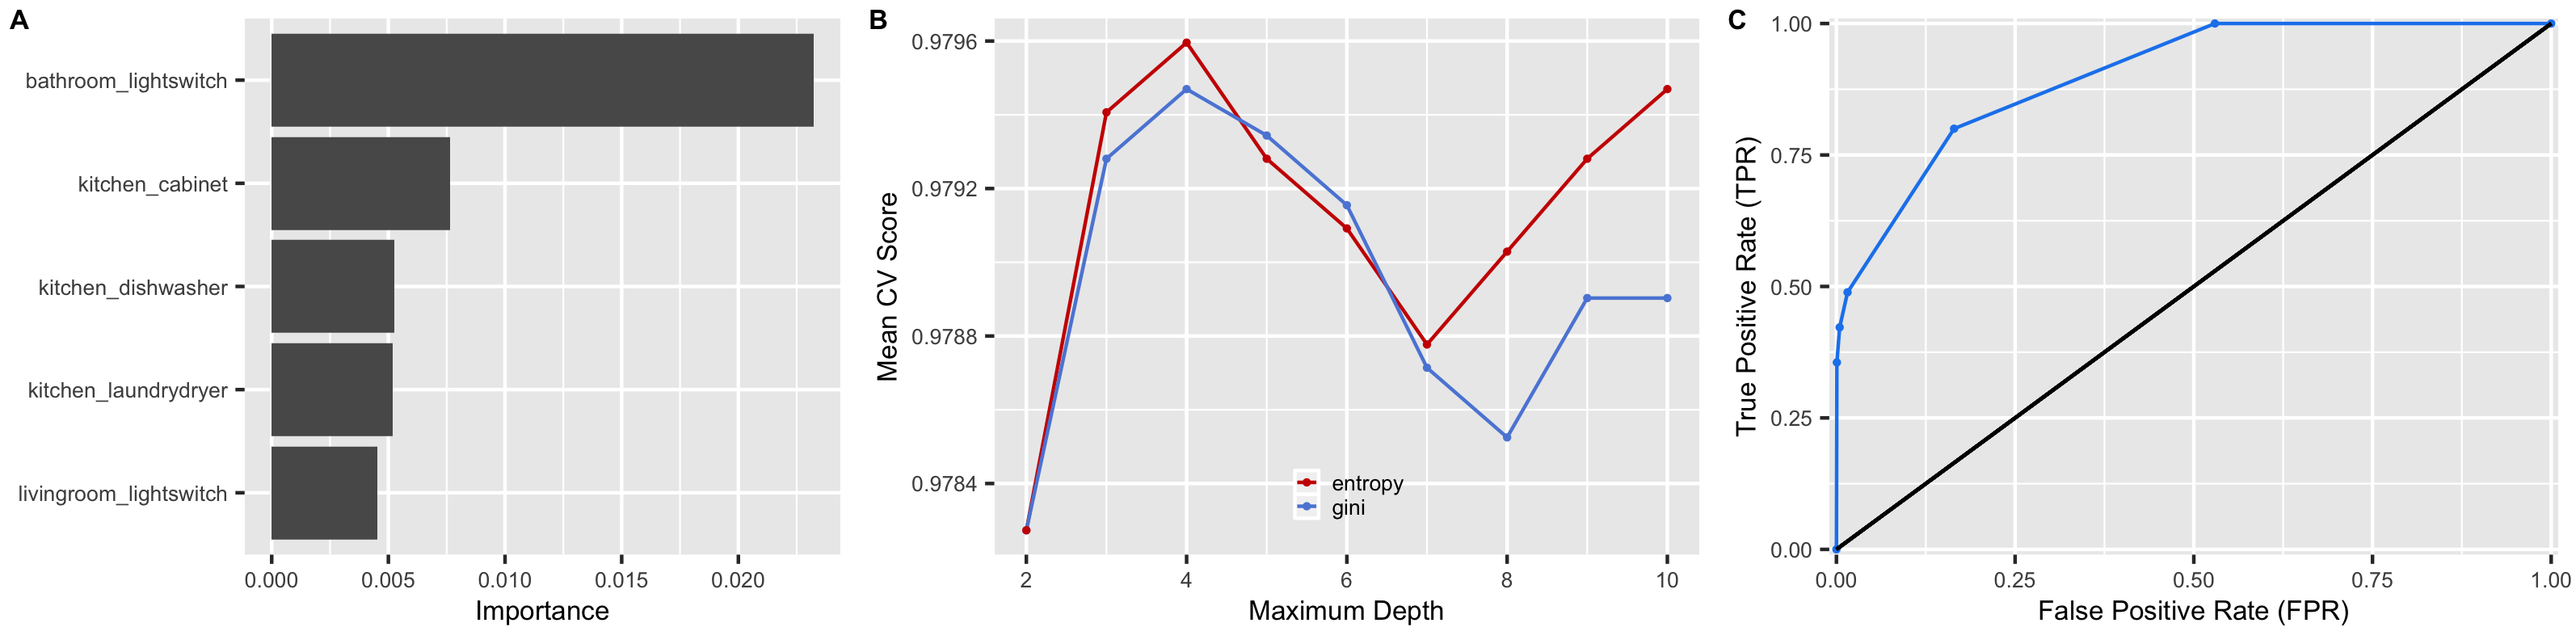
\includegraphics[width=1\linewidth]{/Users/alistairgj/Documents/GitHub/IoT_ResearchProject/IoT_November/images/bedroom_lightswitch_allFeatures} 

}

\caption{ADD TEXT}\label{fig:unnamed-chunk-1}
\end{figure}

\pagebreak

\hypertarget{kitchen-laundrydryer}{%
\subsubsection{Kitchen Laundrydryer}\label{kitchen-laundrydryer}}

\begin{itemize}
\tightlist
\item
  Confusion matrix
\item
  KPIs
\end{itemize}

Fitting 15 folds for each of 18 candidates, totalling 270 fits
\href{Done\%20270\%20out\%20of\%20270\%20\%7C\%20elapsed:\%202.1s\%20finished}{Parallel(n\_jobs=1)}:
Done 270 out of 270 \textbar{} elapsed: 2.1s finished best params:
\{`criterion': `gini', `max\_depth': 5\} best score: 0.988034510989357
precision recall f1-score support

\begin{verbatim}
     0.0       0.99      1.00      0.99      1565
     1.0       0.70      0.30      0.42        23

accuracy                           0.99      1588
\end{verbatim}

macro avg 0.84 0.65 0.71 1588 weighted avg 0.99 0.99 0.99 1588

{[}{[}1562 3{]} {[} 16 7{]}{]} Fitting 15 folds for each of 18
candidates, totalling 270 fits
\href{Done\%20270\%20out\%20of\%20270\%20\%7C\%20elapsed:\%202.1s\%20finished}{Parallel(n\_jobs=1)}:
Using backend SequentialBackend with 1 concurrent workers.
\href{Done\%20270\%20out\%20of\%20270\%20\%7C\%20elapsed:\%202.1s\%20finished}{Parallel(n\_jobs=1)}:
Done 270 out of 270 \textbar{} elapsed: 1.9s finished

\begin{figure}[H]

{\centering 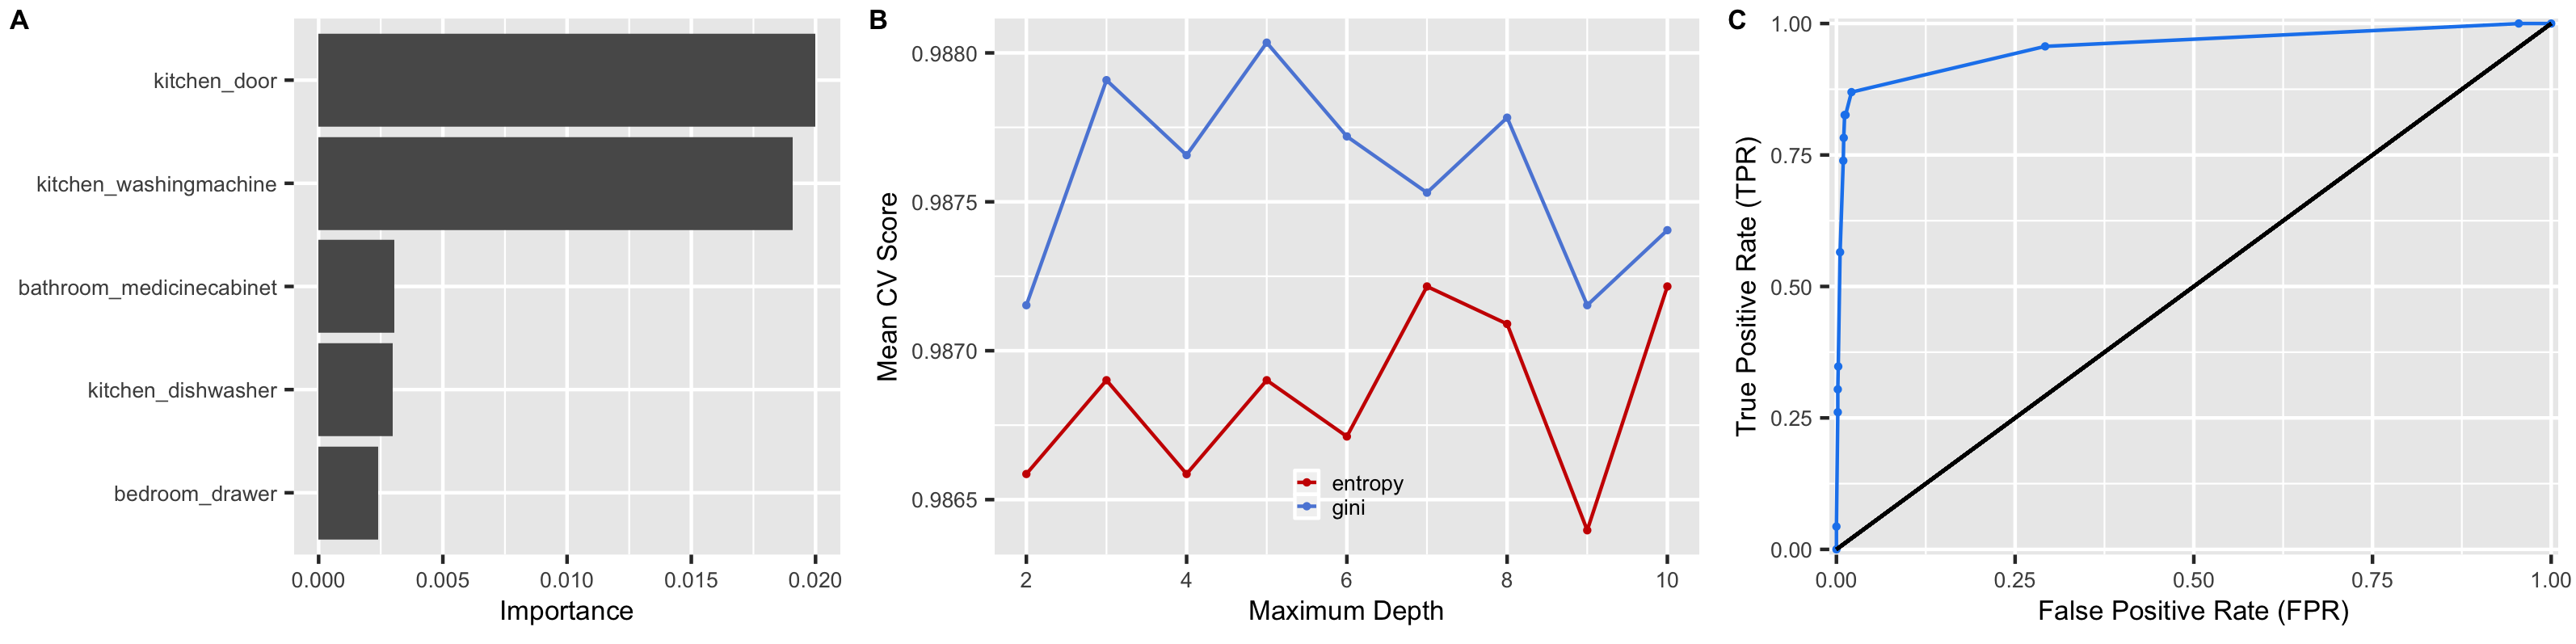
\includegraphics[width=1\linewidth]{/Users/alistairgj/Documents/GitHub/IoT_ResearchProject/IoT_November/images/kitchen_laundrydryer_allFeatures} 

}

\caption{ADD TEXT}\label{fig:unnamed-chunk-2}
\end{figure}

\pagebreak

\hypertarget{kitchen-freezer}{%
\subsubsection{Kitchen Freezer}\label{kitchen-freezer}}

\begin{itemize}
\tightlist
\item
  Confusion matrix
\item
  KPIs
\end{itemize}

Fitting 15 folds for each of 18 candidates, totalling 270 fits
\href{Done\%20270\%20out\%20of\%20270\%20\%7C\%20elapsed:\%202.1s\%20finished}{Parallel(n\_jobs=1)}:
Done 270 out of 270 \textbar{} elapsed: 2.5s finished best params:
\{`criterion': `gini', `max\_depth': 9\} best score: 0.9164305056993514

\begin{verbatim}
       precision    recall  f1-score   support

     0.0       0.94      0.98      0.96      1423
     1.0       0.76      0.44      0.56       165

accuracy                           0.93      1588
\end{verbatim}

macro avg 0.85 0.71 0.76 1588 weighted avg 0.92 0.93 0.92 1588

{[}{[}1400 23{]} {[} 92 73{]}{]} Fitting 15 folds for each of 18
candidates, totalling 270 fits
\href{Done\%20270\%20out\%20of\%20270\%20\%7C\%20elapsed:\%202.1s\%20finished}{Parallel(n\_jobs=1)}:
Using backend SequentialBackend with 1 concurrent workers.
\href{Done\%20270\%20out\%20of\%20270\%20\%7C\%20elapsed:\%202.1s\%20finished}{Parallel(n\_jobs=1)}:
Done 270 out of 270 \textbar{} elapsed: 2.1s finished

\begin{figure}[H]

{\centering 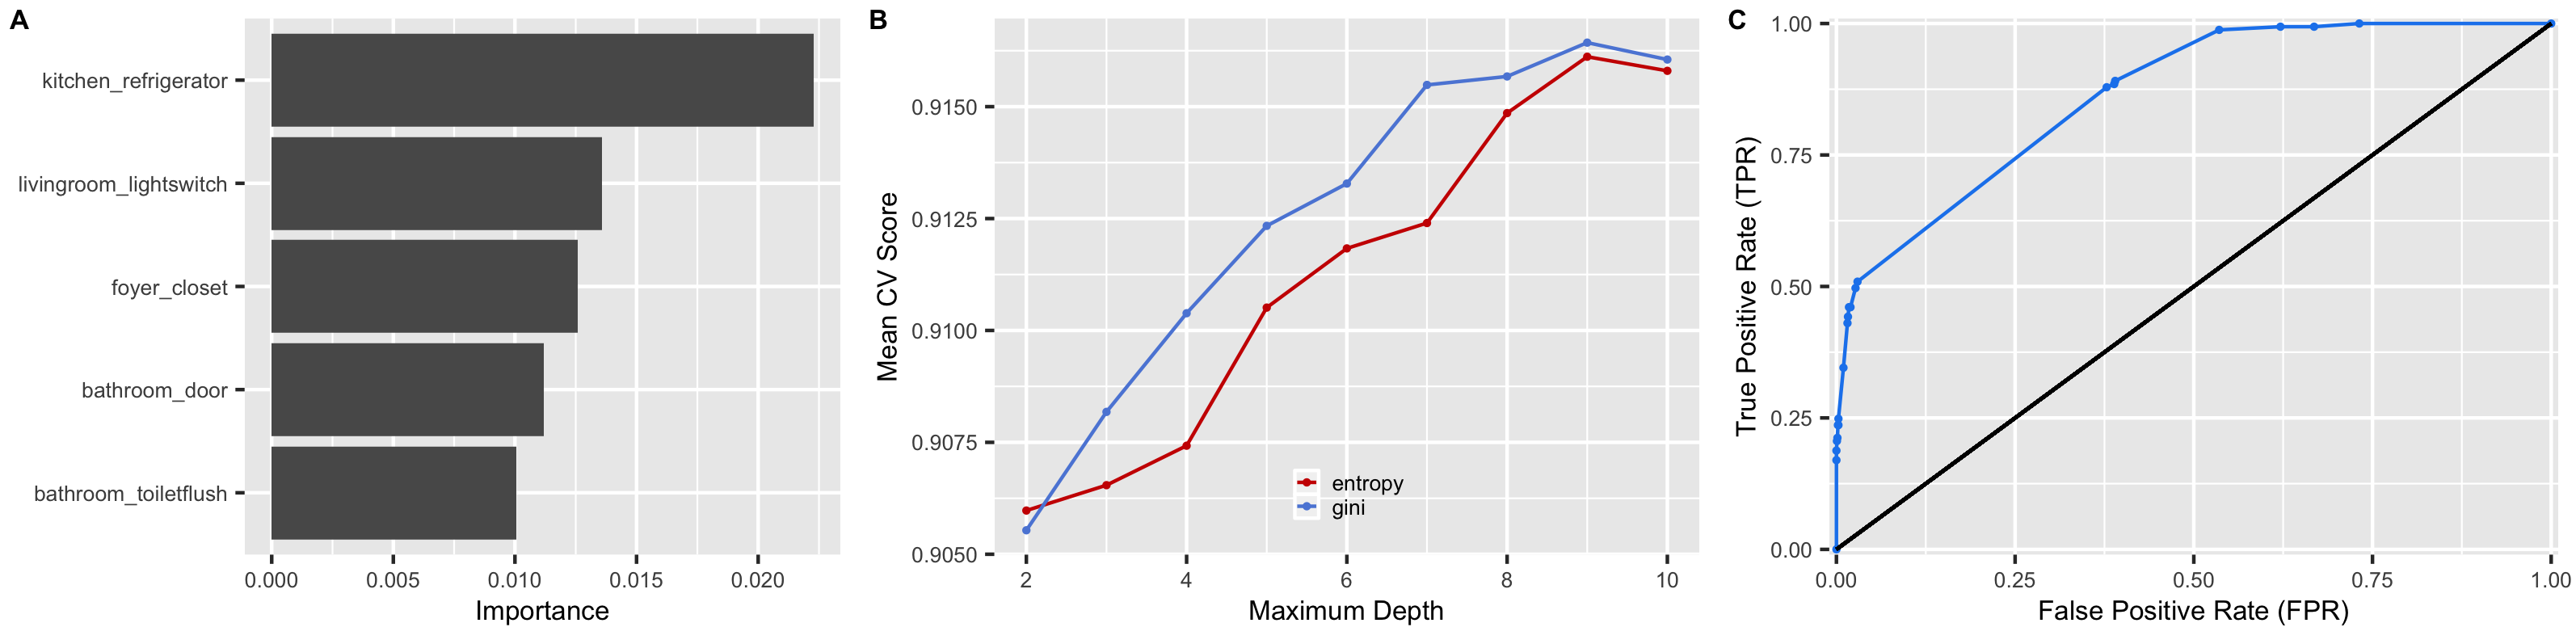
\includegraphics[width=1\linewidth]{/Users/alistairgj/Documents/GitHub/IoT_ResearchProject/IoT_November/images/kitchen_freezer_allFeatures} 

}

\caption{ADD TEXT}\label{fig:unnamed-chunk-3}
\end{figure}

\pagebreak

\hypertarget{kitchen-toaster}{%
\subsubsection{Kitchen Toaster}\label{kitchen-toaster}}

\begin{itemize}
\tightlist
\item
  Confusion matrix
\item
  KPIs
\end{itemize}

Fitting 15 folds for each of 18 candidates, totalling 270 fits
\href{Done\%20270\%20out\%20of\%20270\%20\%7C\%20elapsed:\%202.1s\%20finished}{Parallel(n\_jobs=1)}:
Done 270 out of 270 \textbar{} elapsed: 2.5s finished best params:
\{`criterion': `gini', `max\_depth': 3\} best score: 0.9886642735688645

\begin{verbatim}
  precision    recall  f1-score   support

     0.0       0.99      1.00      0.99      1566
     1.0       0.83      0.23      0.36        22

accuracy                           0.99      1588
\end{verbatim}

macro avg 0.91 0.61 0.68 1588 weighted avg 0.99 0.99 0.99 1588

{[}{[}1565 1{]} {[} 17 5{]}{]} Fitting 15 folds for each of 18
candidates, totalling 270 fits
\href{Done\%20270\%20out\%20of\%20270\%20\%7C\%20elapsed:\%202.1s\%20finished}{Parallel(n\_jobs=1)}:
Using backend SequentialBackend with 1 concurrent workers.
\href{Done\%20270\%20out\%20of\%20270\%20\%7C\%20elapsed:\%202.1s\%20finished}{Parallel(n\_jobs=1)}:
Done 270 out of 270 \textbar{} elapsed: 2.7s finished

\begin{figure}[H]

{\centering 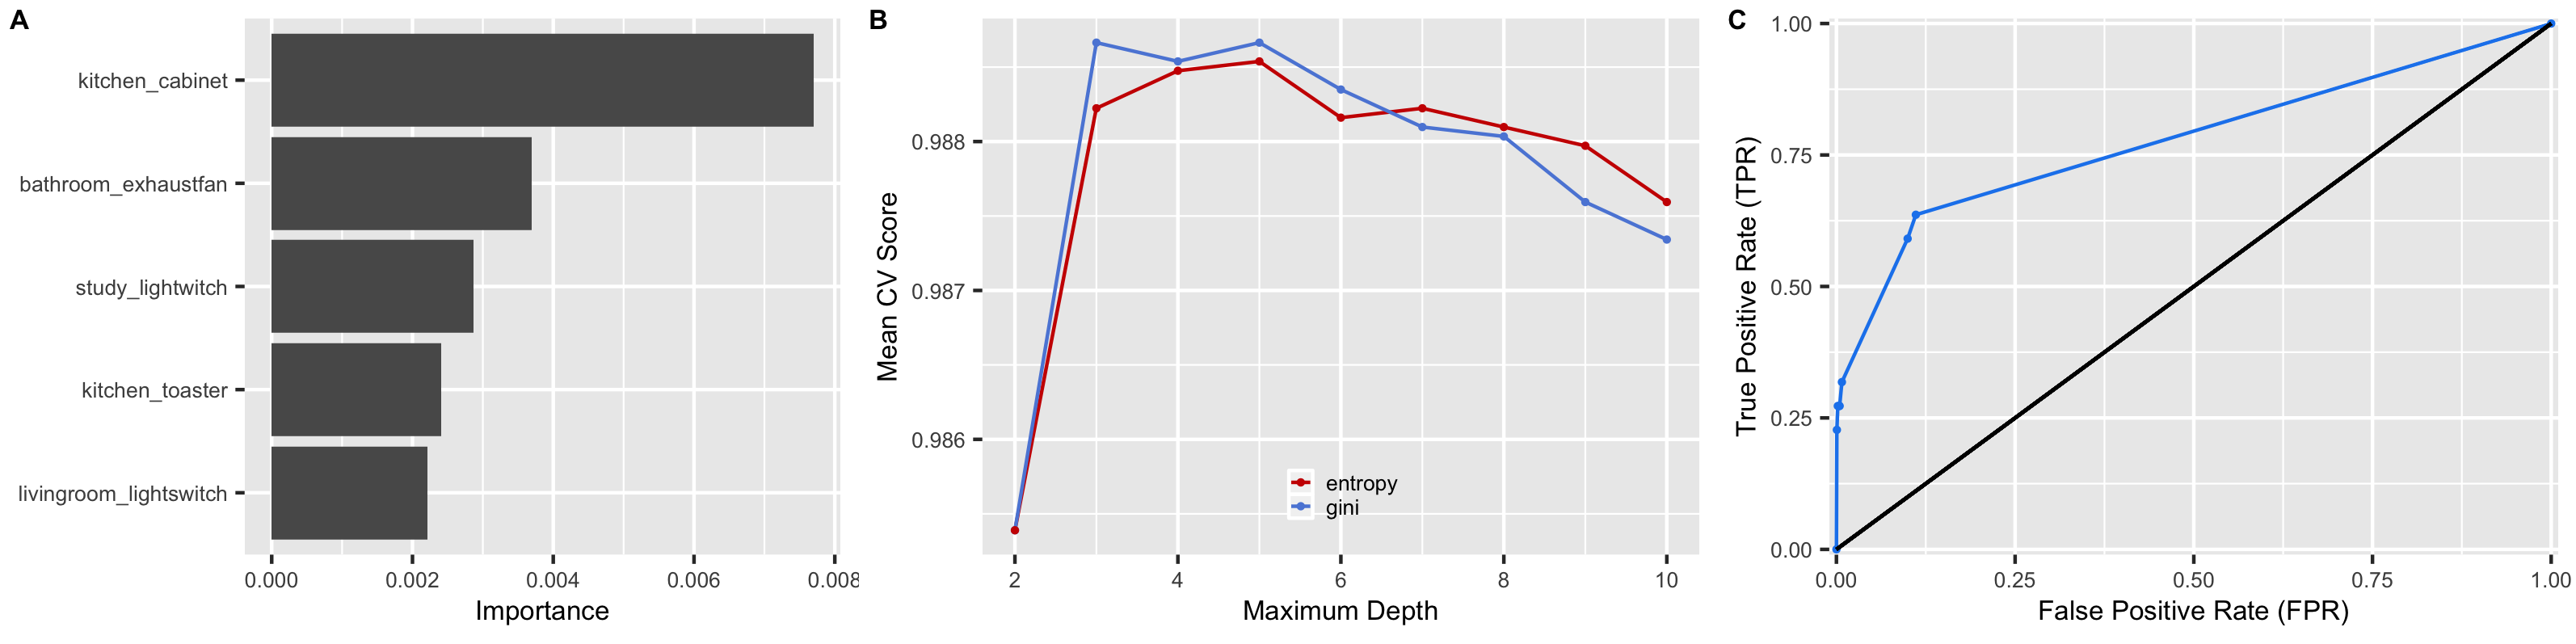
\includegraphics[width=1\linewidth]{/Users/alistairgj/Documents/GitHub/IoT_ResearchProject/IoT_November/images/kitchen_toaster_allFeatures} 

}

\caption{ADD TEXT}\label{fig:unnamed-chunk-4}
\end{figure}

\pagebreak

\hypertarget{bathroom-exhaustfan}{%
\subsubsection{Bathroom Exhaustfan}\label{bathroom-exhaustfan}}

\begin{itemize}
\tightlist
\item
  Confusion matrix
\item
  KPIs
\end{itemize}

Fitting 15 folds for each of 18 candidates, totalling 270 fits
\href{Done\%20270\%20out\%20of\%20270\%20\%7C\%20elapsed:\%202.1s\%20finished}{Parallel(n\_jobs=1)}:
Done 270 out of 270 \textbar{} elapsed: 2.3s finished best params:
\{`criterion': `gini', `max\_depth': 8\} best score: 0.8798412998299641

\begin{verbatim}
  precision    recall  f1-score   support

     0.0       0.90      0.99      0.94      1384
     1.0       0.77      0.25      0.38       204

accuracy                           0.89      1588
\end{verbatim}

macro avg 0.84 0.62 0.66 1588 weighted avg 0.88 0.89 0.87 1588

{[}{[}1369 15{]} {[} 153 51{]}{]} Fitting 15 folds for each of 18
candidates, totalling 270 fits
\href{Done\%20270\%20out\%20of\%20270\%20\%7C\%20elapsed:\%202.1s\%20finished}{Parallel(n\_jobs=1)}:
Using backend SequentialBackend with 1 concurrent workers.
\href{Done\%20270\%20out\%20of\%20270\%20\%7C\%20elapsed:\%202.1s\%20finished}{Parallel(n\_jobs=1)}:
Done 270 out of 270 \textbar{} elapsed: 2.9s finished

\begin{figure}[H]

{\centering 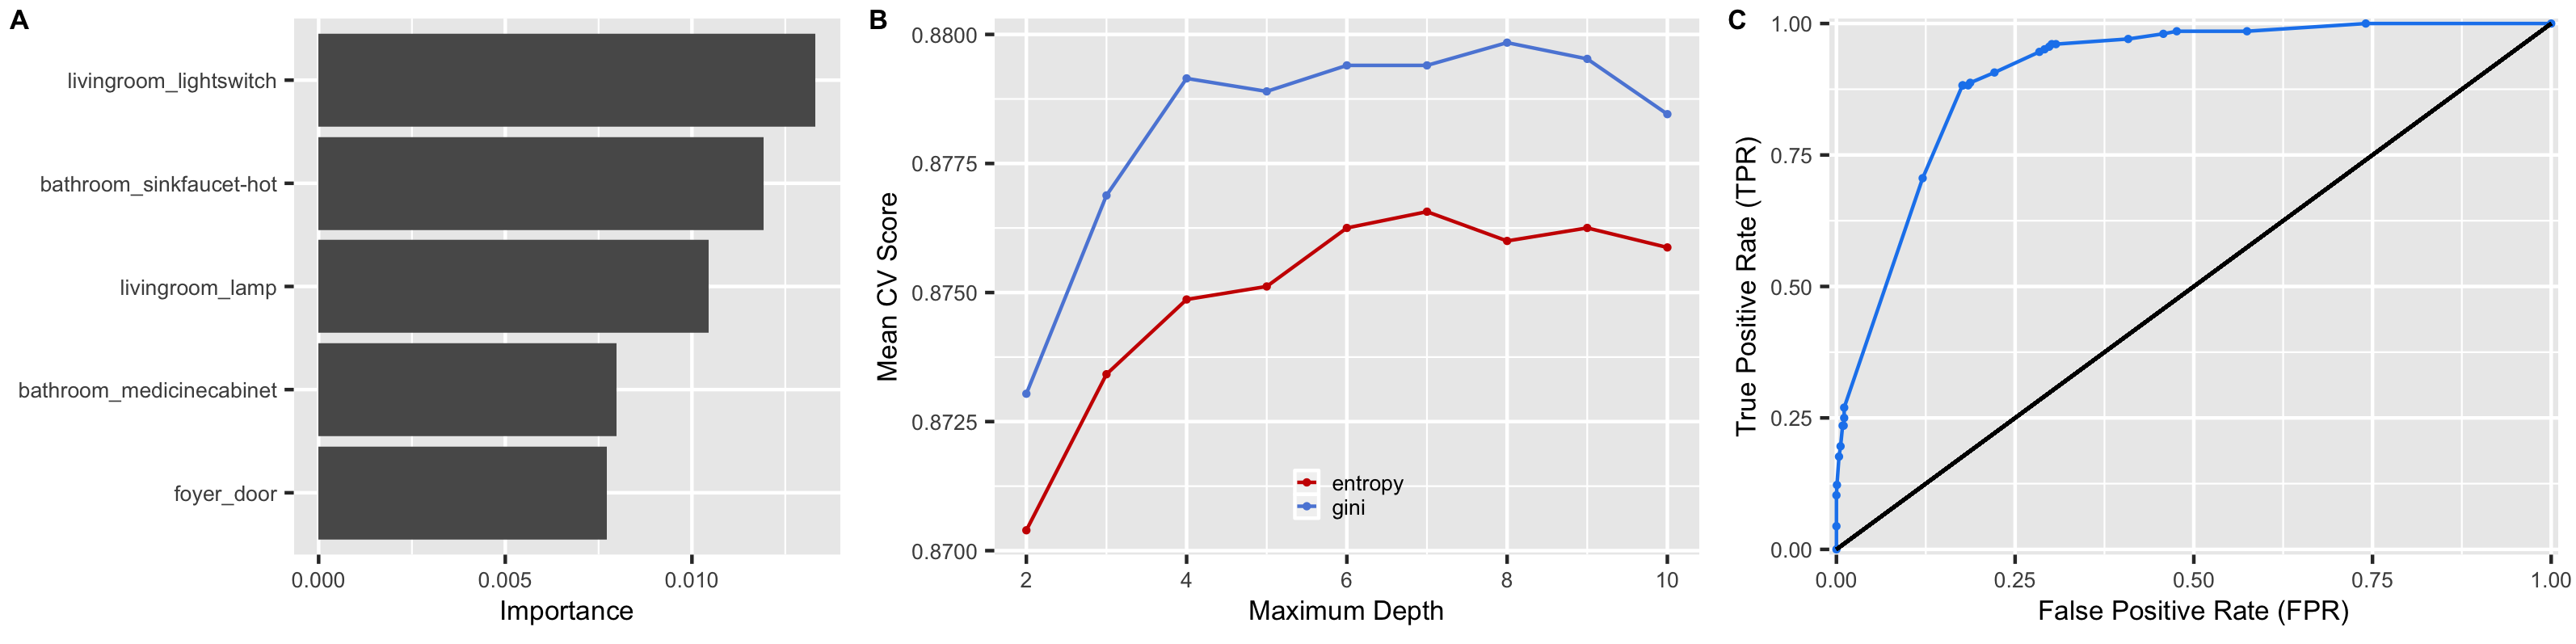
\includegraphics[width=1\linewidth]{/Users/alistairgj/Documents/GitHub/IoT_ResearchProject/IoT_November/images/bathroom_exhaustfan_allFeatures} 

}

\caption{ADD TEXT}\label{fig:unnamed-chunk-5}
\end{figure}

\pagebreak

\hypertarget{bathroom-showerfaucet}{%
\subsubsection{Bathroom Showerfaucet}\label{bathroom-showerfaucet}}

\begin{itemize}
\tightlist
\item
  Confusion matrix
\item
  KPIs
\end{itemize}

Fitting 15 folds for each of 18 candidates, totalling 270 fits
\href{Done\%20270\%20out\%20of\%20270\%20\%7C\%20elapsed:\%202.1s\%20finished}{Parallel(n\_jobs=1)}:
Done 270 out of 270 \textbar{} elapsed: 2.5s finished best params:
\{`criterion': `entropy', `max\_depth': 8\} best score:
0.9669374645758549

\begin{verbatim}
      precision    recall  f1-score   support

     0.0       0.97      1.00      0.98      1520
     1.0       0.82      0.40      0.53        68

accuracy                           0.97      1588
\end{verbatim}

macro avg 0.90 0.70 0.76 1588 weighted avg 0.97 0.97 0.97 1588

{[}{[}1514 6{]} {[} 41 27{]}{]} Fitting 15 folds for each of 18
candidates, totalling 270 fits
\href{Done\%20270\%20out\%20of\%20270\%20\%7C\%20elapsed:\%202.1s\%20finished}{Parallel(n\_jobs=1)}:
Using backend SequentialBackend with 1 concurrent workers.
\href{Done\%20270\%20out\%20of\%20270\%20\%7C\%20elapsed:\%202.1s\%20finished}{Parallel(n\_jobs=1)}:
Done 270 out of 270 \textbar{} elapsed: 2.7s finished

\begin{figure}[H]

{\centering 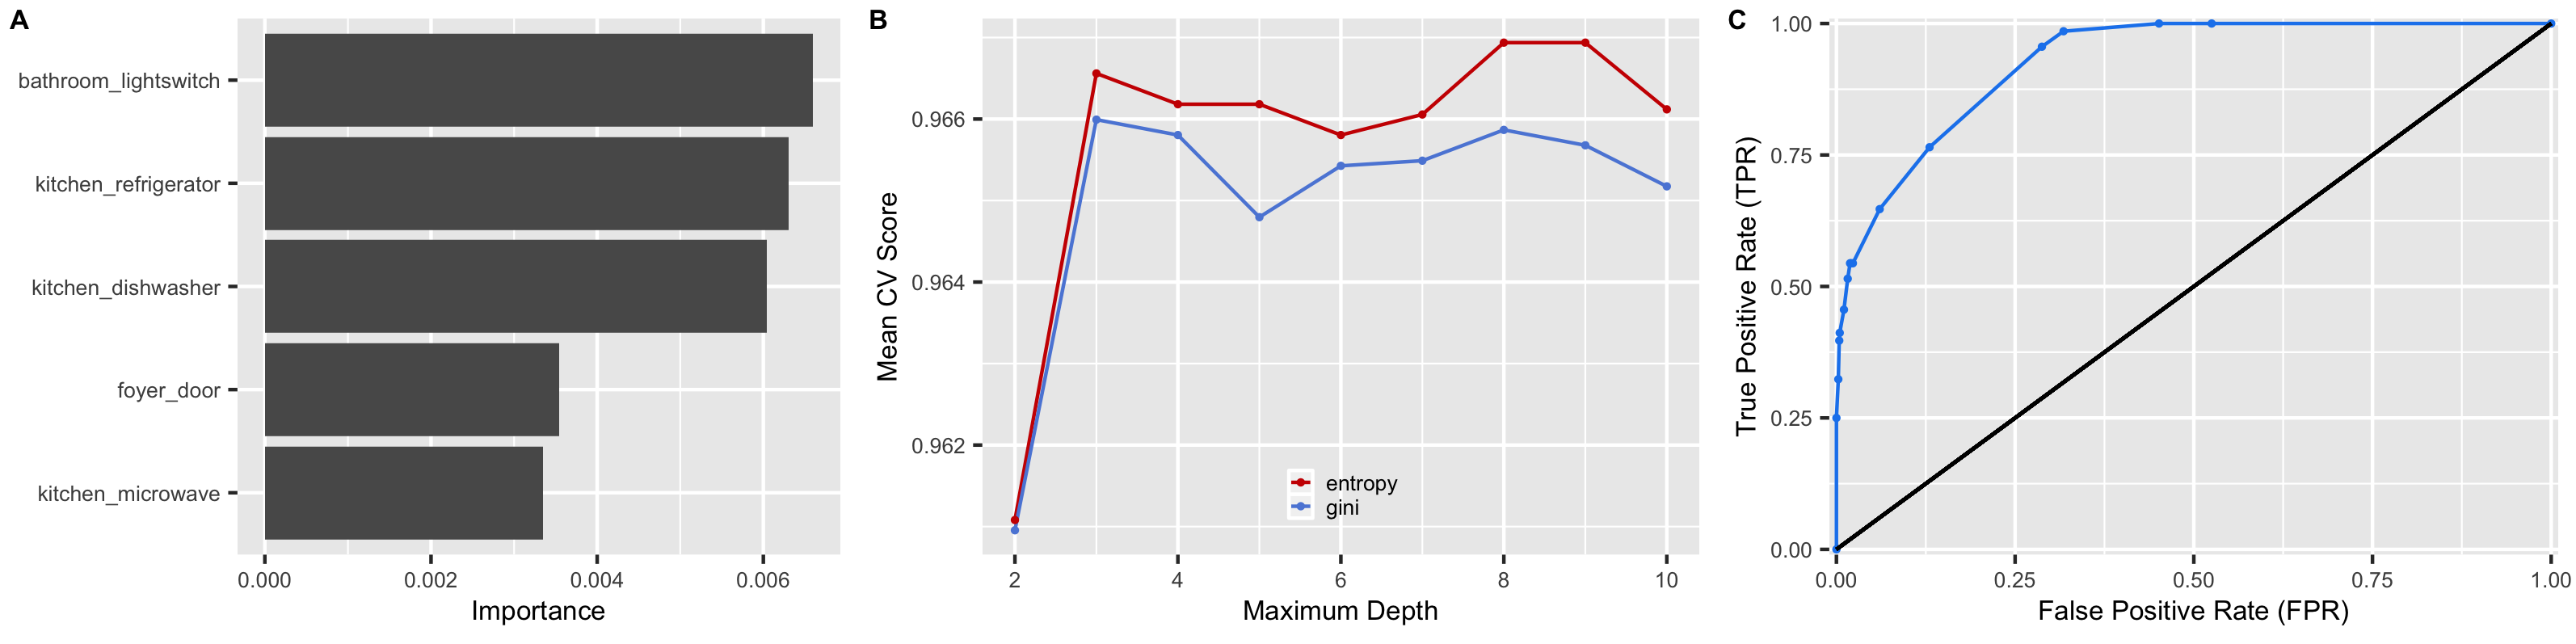
\includegraphics[width=1\linewidth]{/Users/alistairgj/Documents/GitHub/IoT_ResearchProject/IoT_November/images/bathroom_showerfaucet_allFeatures} 

}

\caption{ADD TEXT}\label{fig:unnamed-chunk-6}
\end{figure}

\pagebreak

\hypertarget{bathroom_lightswitch}{%
\subsubsection{bathroom\_lightswitch}\label{bathroom_lightswitch}}

\begin{itemize}
\tightlist
\item
  Confusion matrix
\item
  KPIs
\end{itemize}

Fitting 15 folds for each of 18 candidates, totalling 270 fits
\href{Done\%20270\%20out\%20of\%20270\%20\%7C\%20elapsed:\%202.1s\%20finished}{Parallel(n\_jobs=1)}:
Done 270 out of 270 \textbar{} elapsed: 2.5s finished best params:
\{`criterion': `gini', `max\_depth': 10\} best score: 0.8392216134517287

\begin{verbatim}
    precision    recall  f1-score   support

     0.0       0.85      0.99      0.91      1262
     1.0       0.85      0.30      0.45       326

accuracy                           0.85      1588
\end{verbatim}

macro avg 0.85 0.64 0.68 1588 weighted avg 0.85 0.85 0.82 1588

{[}{[}1244 18{]} {[} 227 99{]}{]} Fitting 15 folds for each of 18
candidates, totalling 270 fits
\href{Done\%20270\%20out\%20of\%20270\%20\%7C\%20elapsed:\%202.1s\%20finished}{Parallel(n\_jobs=1)}:
Using backend SequentialBackend with 1 concurrent workers.
\href{Done\%20270\%20out\%20of\%20270\%20\%7C\%20elapsed:\%202.1s\%20finished}{Parallel(n\_jobs=1)}:
Done 270 out of 270 \textbar{} elapsed: 3.0s finished

\begin{figure}[H]

{\centering 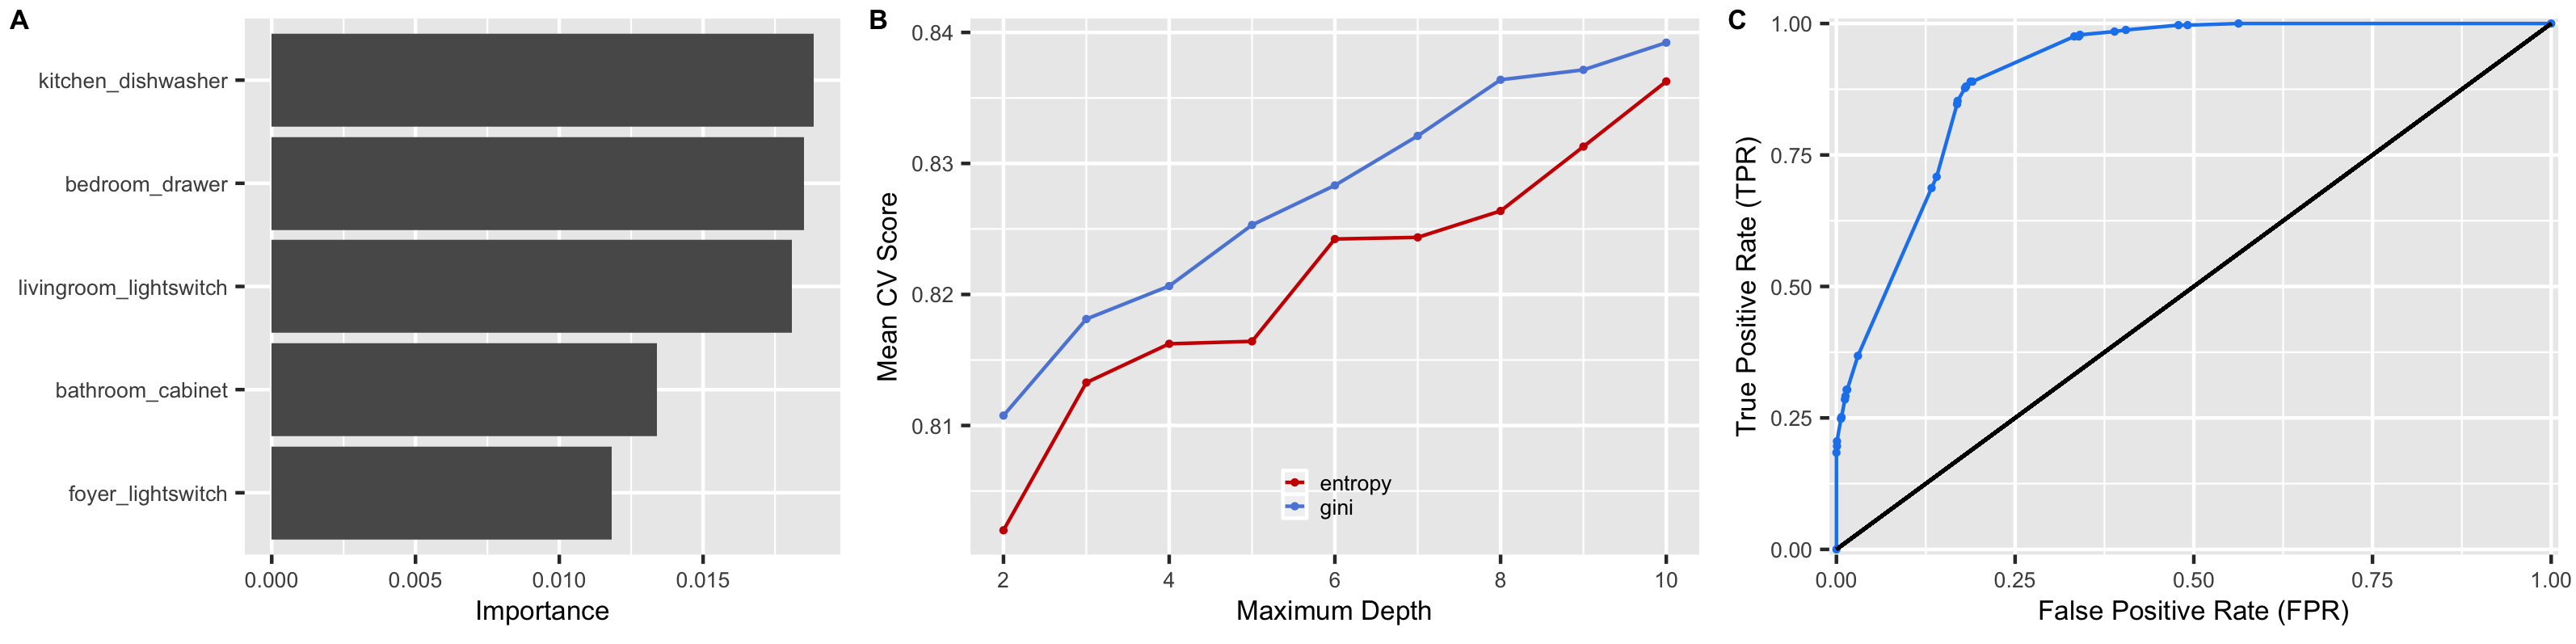
\includegraphics[width=1\linewidth]{/Users/alistairgj/Documents/GitHub/IoT_ResearchProject/IoT_November/images/bathroom_lightswitch_allFeatures} 

}

\caption{ADD TEXT}\label{fig:unnamed-chunk-7}
\end{figure}

\pagebreak

\hypertarget{kitchen_refrigerator}{%
\subsubsection{kitchen\_refrigerator}\label{kitchen_refrigerator}}

\begin{itemize}
\tightlist
\item
  Confusion matrix
\item
  KPIs
\end{itemize}

Fitting 15 folds for each of 18 candidates, totalling 270 fits
\href{Done\%20270\%20out\%20of\%20270\%20\%7C\%20elapsed:\%202.1s\%20finished}{Parallel(n\_jobs=1)}:
Done 270 out of 270 \textbar{} elapsed: 3.0s finished best params:
\{`criterion': `gini', `max\_depth': 10\} best score: 0.9646073430316771

\begin{verbatim}
  precision    recall  f1-score   support

     0.0       0.97      1.00      0.99      1506
     1.0       0.95      0.51      0.67        82

accuracy                           0.97      1588
\end{verbatim}

macro avg 0.96 0.76 0.83 1588 weighted avg 0.97 0.97 0.97 1588

{[}{[}1504 2{]} {[} 40 42{]}{]} Fitting 15 folds for each of 18
candidates, totalling 270 fits
\href{Done\%20270\%20out\%20of\%20270\%20\%7C\%20elapsed:\%202.1s\%20finished}{Parallel(n\_jobs=1)}:
Using backend SequentialBackend with 1 concurrent workers.
\href{Done\%20270\%20out\%20of\%20270\%20\%7C\%20elapsed:\%202.1s\%20finished}{Parallel(n\_jobs=1)}:
Done 270 out of 270 \textbar{} elapsed: 2.4s finished

\begin{figure}[H]

{\centering 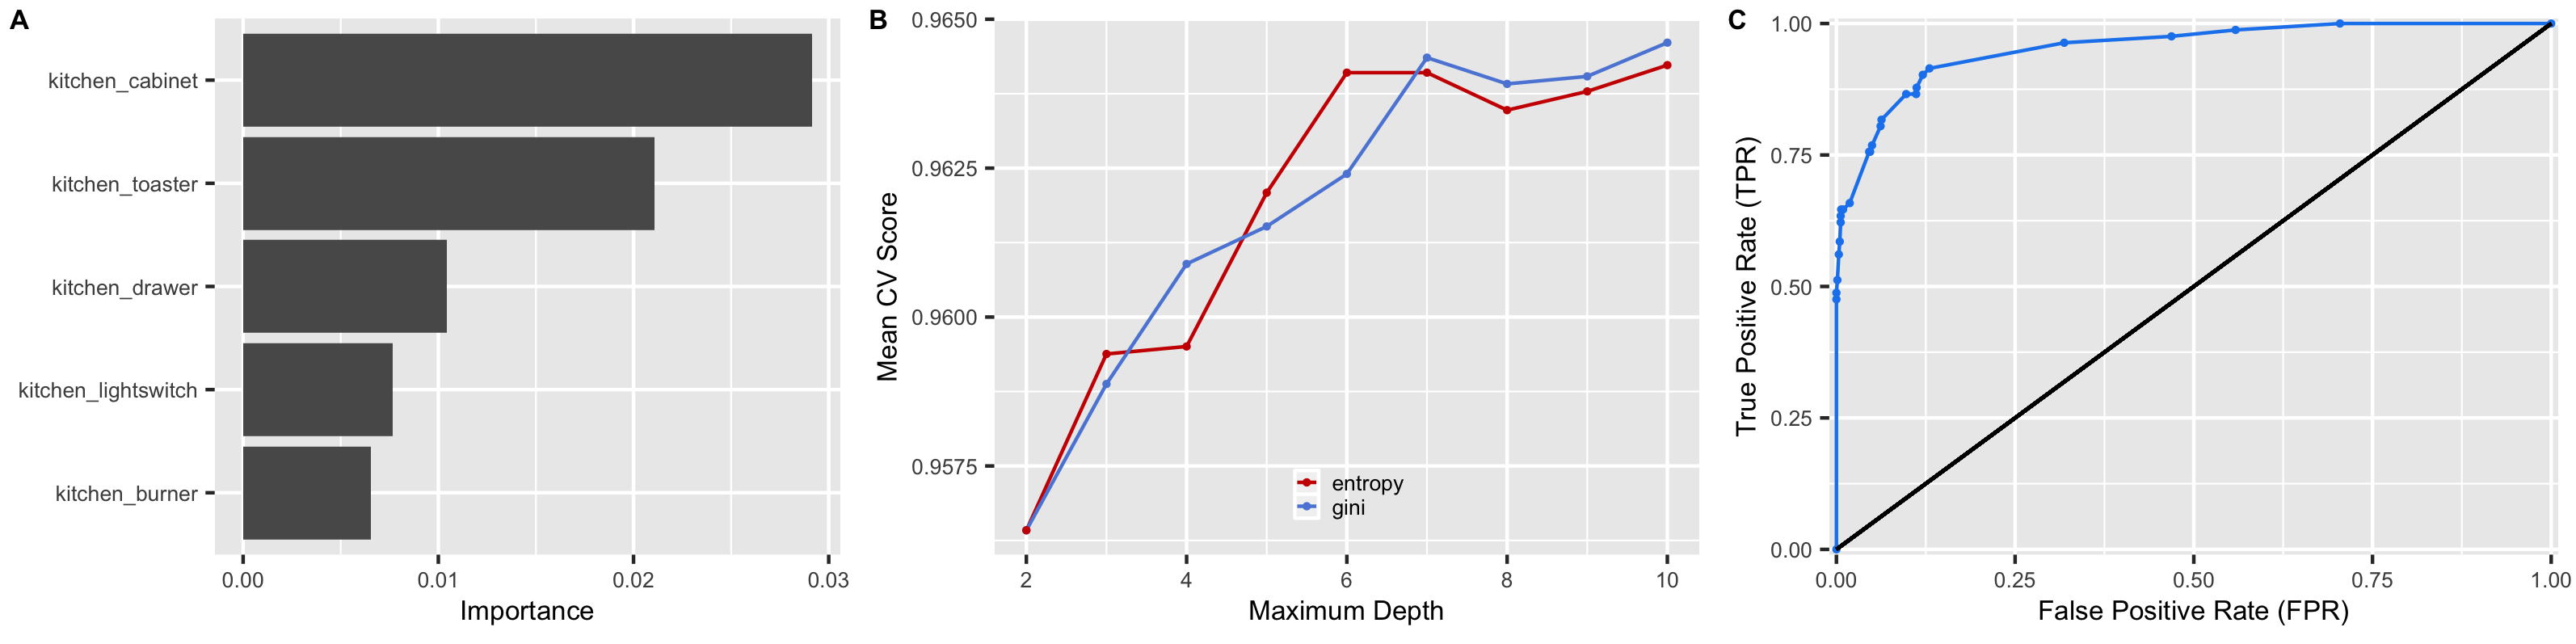
\includegraphics[width=1\linewidth]{/Users/alistairgj/Documents/GitHub/IoT_ResearchProject/IoT_November/images/kitchen_refrigerator_allFeatures} 

}

\caption{ADD TEXT}\label{fig:unnamed-chunk-8}
\end{figure}

\pagebreak

\hypertarget{foyer_lightswitch}{%
\subsubsection{foyer\_lightswitch}\label{foyer_lightswitch}}

\begin{itemize}
\tightlist
\item
  Confusion matrix
\item
  KPIs
\end{itemize}

Fitting 15 folds for each of 18 candidates, totalling 270 fits
\href{Done\%20270\%20out\%20of\%20270\%20\%7C\%20elapsed:\%202.1s\%20finished}{Parallel(n\_jobs=1)}:
Done 270 out of 270 \textbar{} elapsed: 2.9s finished best params:
\{`criterion': `gini', `max\_depth': 4\} best score: 0.9894199886642736

\begin{verbatim}
     precision    recall  f1-score   support

     0.0       0.99      1.00      1.00      1528
     1.0       0.98      0.77      0.86        60

accuracy                           0.99      1588
\end{verbatim}

macro avg 0.98 0.88 0.93 1588 weighted avg 0.99 0.99 0.99 1588

{[}{[}1527 1{]} {[} 14 46{]}{]} Fitting 15 folds for each of 18
candidates, totalling 270 fits
\href{Done\%20270\%20out\%20of\%20270\%20\%7C\%20elapsed:\%202.1s\%20finished}{Parallel(n\_jobs=1)}:
Using backend SequentialBackend with 1 concurrent workers.
\href{Done\%20270\%20out\%20of\%20270\%20\%7C\%20elapsed:\%202.1s\%20finished}{Parallel(n\_jobs=1)}:
Done 270 out of 270 \textbar{} elapsed: 3.0s finished

\begin{figure}[H]

{\centering 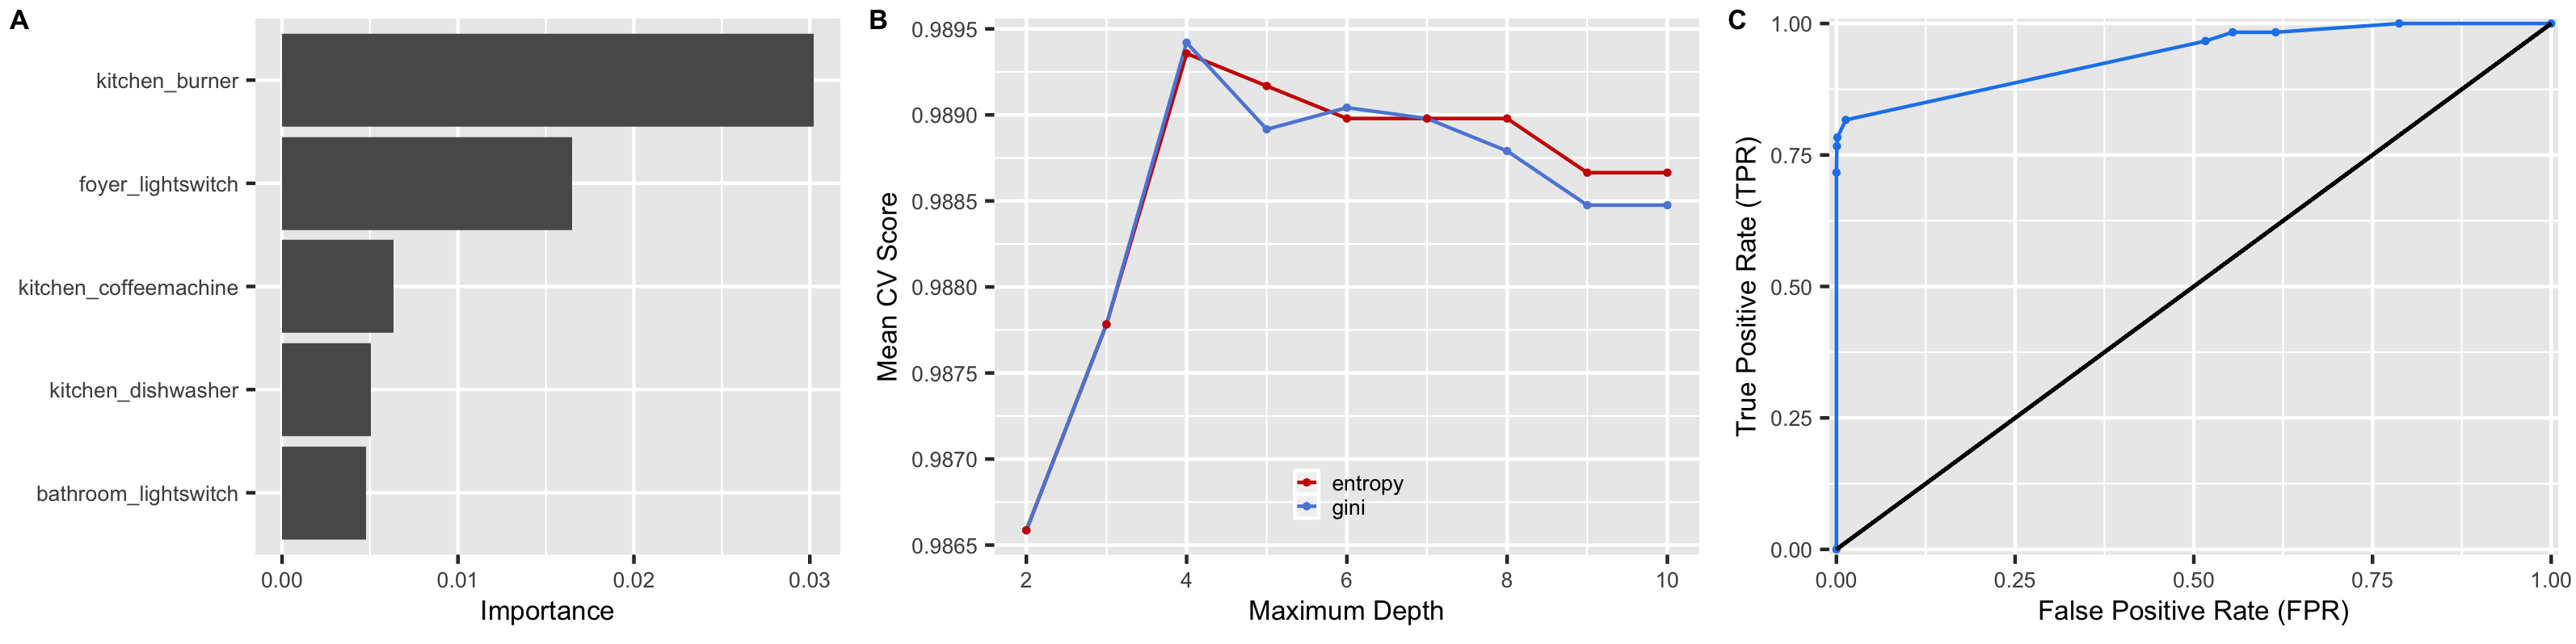
\includegraphics[width=1\linewidth]{/Users/alistairgj/Documents/GitHub/IoT_ResearchProject/IoT_November/images/foyer_lightswitch_allFeatures} 

}

\caption{ADD TEXT}\label{fig:unnamed-chunk-9}
\end{figure}

\pagebreak

\hypertarget{kitchen_burner}{%
\subsubsection{kitchen\_burner}\label{kitchen_burner}}

\begin{itemize}
\tightlist
\item
  Confusion matrix
\item
  KPIs
\end{itemize}

Fitting 15 folds for each of 18 candidates, totalling 270 fits
\href{Done\%20270\%20out\%20of\%20270\%20\%7C\%20elapsed:\%202.1s\%20finished}{Parallel(n\_jobs=1)}:
Done 270 out of 270 \textbar{} elapsed: 2.5s finished best params:
\{`criterion': `entropy', `max\_depth': 8\} best score:
0.9630329365829082

\begin{verbatim}
 precision    recall  f1-score   support

     0.0       0.97      1.00      0.98      1506
     1.0       0.97      0.34      0.50        82

accuracy                           0.97      1588
\end{verbatim}

macro avg 0.97 0.67 0.74 1588 weighted avg 0.97 0.97 0.96 1588

{[}{[}1505 1{]} {[} 54 28{]}{]} Fitting 15 folds for each of 18
candidates, totalling 270 fits
\href{Done\%20270\%20out\%20of\%20270\%20\%7C\%20elapsed:\%202.1s\%20finished}{Parallel(n\_jobs=1)}:
Using backend SequentialBackend with 1 concurrent workers.
\href{Done\%20270\%20out\%20of\%20270\%20\%7C\%20elapsed:\%202.1s\%20finished}{Parallel(n\_jobs=1)}:
Done 270 out of 270 \textbar{} elapsed: 3.2s finished

\begin{figure}[H]

{\centering 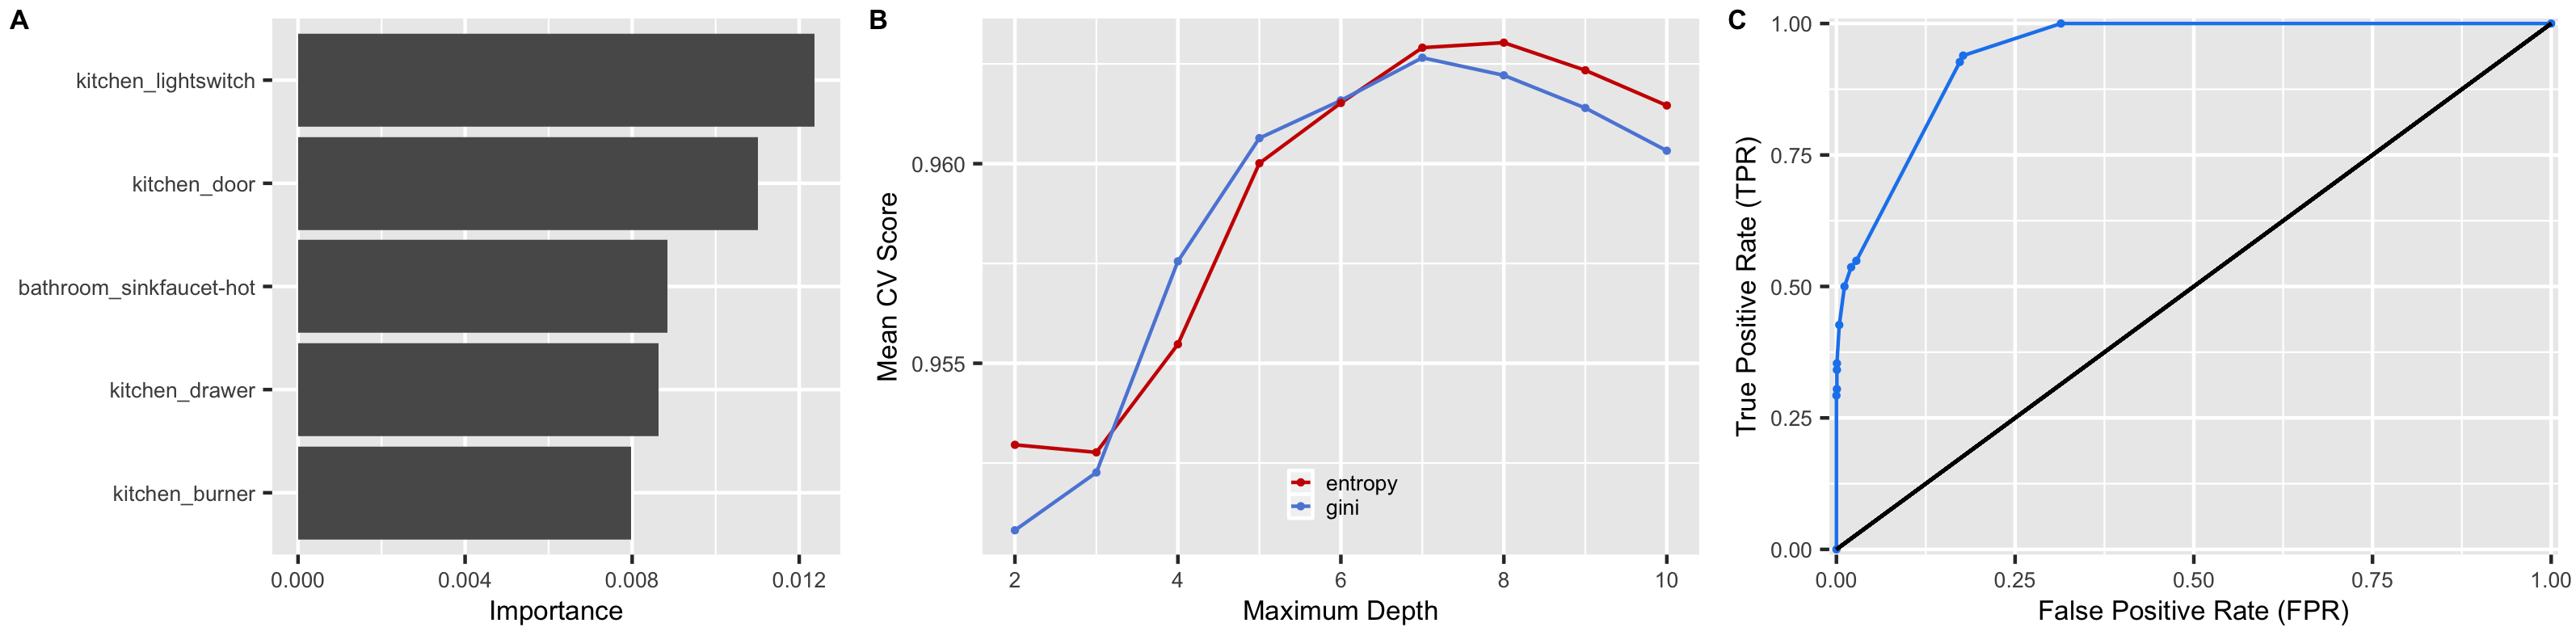
\includegraphics[width=1\linewidth]{/Users/alistairgj/Documents/GitHub/IoT_ResearchProject/IoT_November/images/kitchen_burner_allFeatures} 

}

\caption{ADD TEXT}\label{fig:unnamed-chunk-10}
\end{figure}

\pagebreak

\hypertarget{study-lightswitch}{%
\subsubsection{study Lightswitch}\label{study-lightswitch}}

\begin{itemize}
\tightlist
\item
  Confusion matrix
\item
  KPIs
\end{itemize}

Fitting 15 folds for each of 18 candidates, totalling 270 fits
\href{Done\%20270\%20out\%20of\%20270\%20\%7C\%20elapsed:\%202.1s\%20finished}{Parallel(n\_jobs=1)}:
Done 270 out of 270 \textbar{} elapsed: 2.9s finished best params:
\{`criterion': `entropy', `max\_depth': 8\} best score:
0.8873354745261036

\begin{verbatim}
     precision    recall  f1-score   support

     0.0       0.89      1.00      0.94      1407
     1.0       0.81      0.07      0.13       181

accuracy                           0.89      1588
\end{verbatim}

macro avg 0.85 0.53 0.54 1588 weighted avg 0.88 0.89 0.85 1588

{[}{[}1404 3{]} {[} 168 13{]}{]} Fitting 15 folds for each of 18
candidates, totalling 270 fits
\href{Done\%20270\%20out\%20of\%20270\%20\%7C\%20elapsed:\%202.1s\%20finished}{Parallel(n\_jobs=1)}:
Using backend SequentialBackend with 1 concurrent workers.
\href{Done\%20270\%20out\%20of\%20270\%20\%7C\%20elapsed:\%202.1s\%20finished}{Parallel(n\_jobs=1)}:
Done 270 out of 270 \textbar{} elapsed: 3.3s finished

\begin{figure}[H]

{\centering 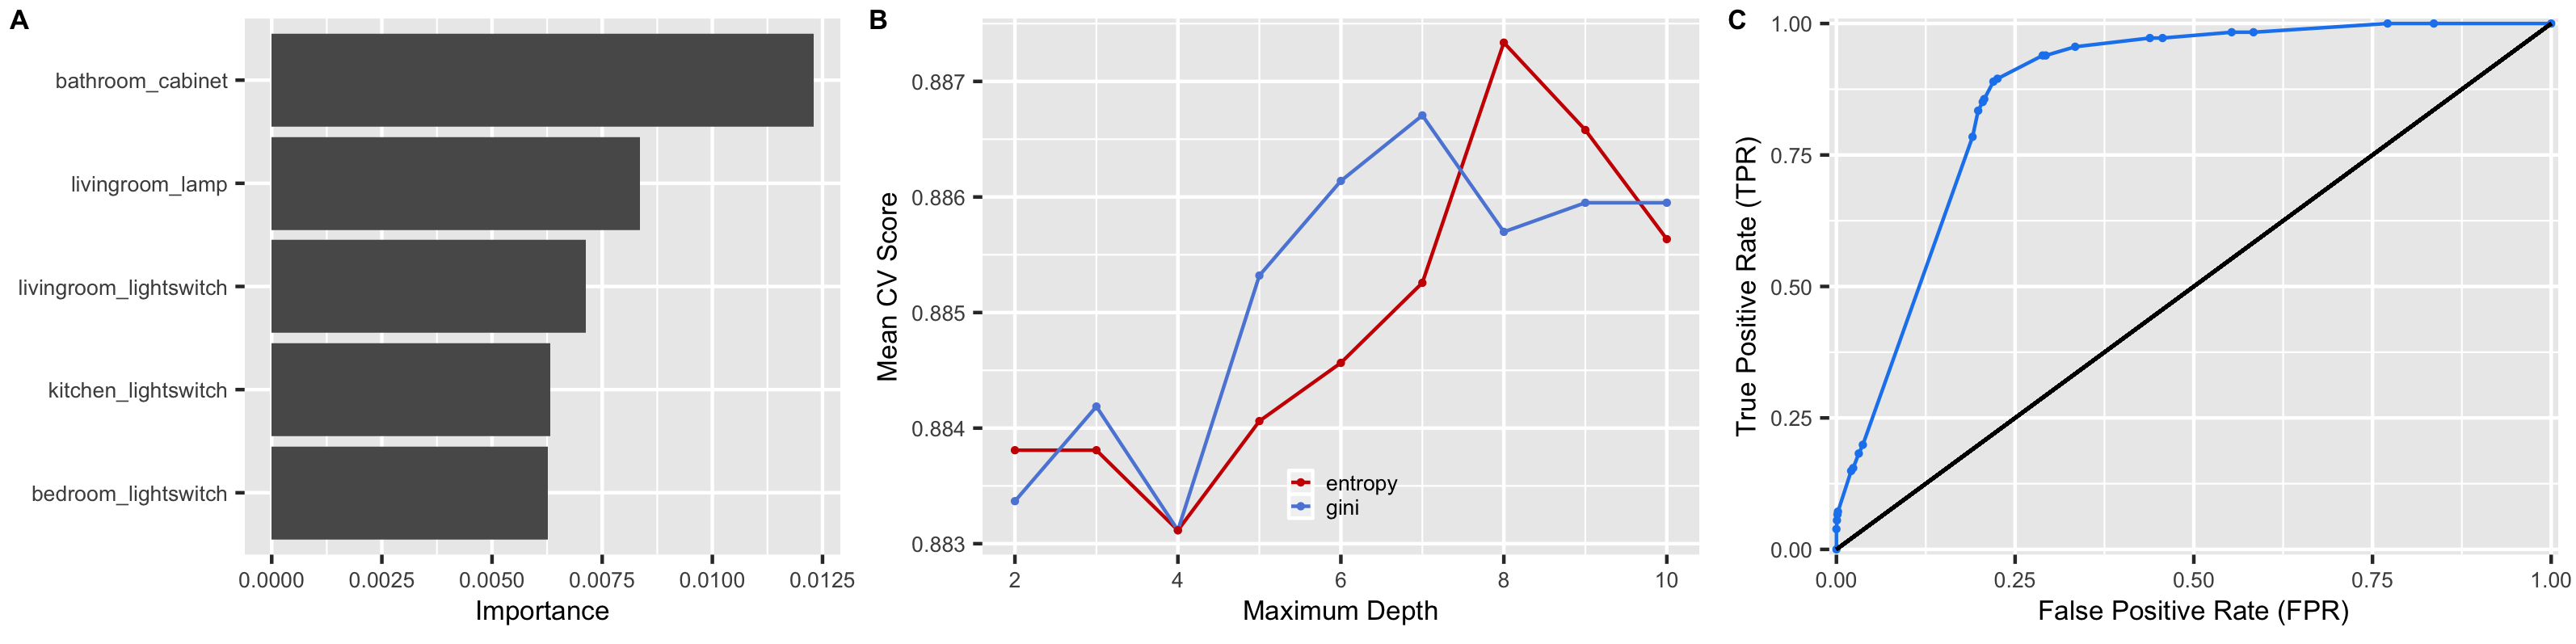
\includegraphics[width=1\linewidth]{/Users/alistairgj/Documents/GitHub/IoT_ResearchProject/IoT_November/images/study_lightwitch_allFeatures} 

}

\caption{ADD TEXT}\label{fig:unnamed-chunk-11}
\end{figure}

\pagebreak

\hypertarget{kitchen_washingmachine}{%
\subsubsection{kitchen\_washingmachine}\label{kitchen_washingmachine}}

\begin{itemize}
\tightlist
\item
  Confusion matrix
\item
  KPIs
\end{itemize}

Fitting 15 folds for each of 18 candidates, totalling 270 fits
\href{Done\%20270\%20out\%20of\%20270\%20\%7C\%20elapsed:\%202.1s\%20finished}{Parallel(n\_jobs=1)}:
Done 270 out of 270 \textbar{} elapsed: 3.1s finished best params:
\{`criterion': `gini', `max\_depth': 3\} best score: 0.9892310598904213

\begin{verbatim}
 precision    recall  f1-score   support

     0.0       0.99      1.00      0.99      1562
     1.0       0.83      0.19      0.31        26

accuracy                           0.99      1588
\end{verbatim}

macro avg 0.91 0.60 0.65 1588 weighted avg 0.98 0.99 0.98 1588

{[}{[}1561 1{]} {[} 21 5{]}{]} Fitting 15 folds for each of 18
candidates, totalling 270 fits
\href{Done\%20270\%20out\%20of\%20270\%20\%7C\%20elapsed:\%202.1s\%20finished}{Parallel(n\_jobs=1)}:
Using backend SequentialBackend with 1 concurrent workers.
\href{Done\%20270\%20out\%20of\%20270\%20\%7C\%20elapsed:\%202.1s\%20finished}{Parallel(n\_jobs=1)}:
Done 270 out of 270 \textbar{} elapsed: 3.0s finished

\begin{figure}[H]

{\centering 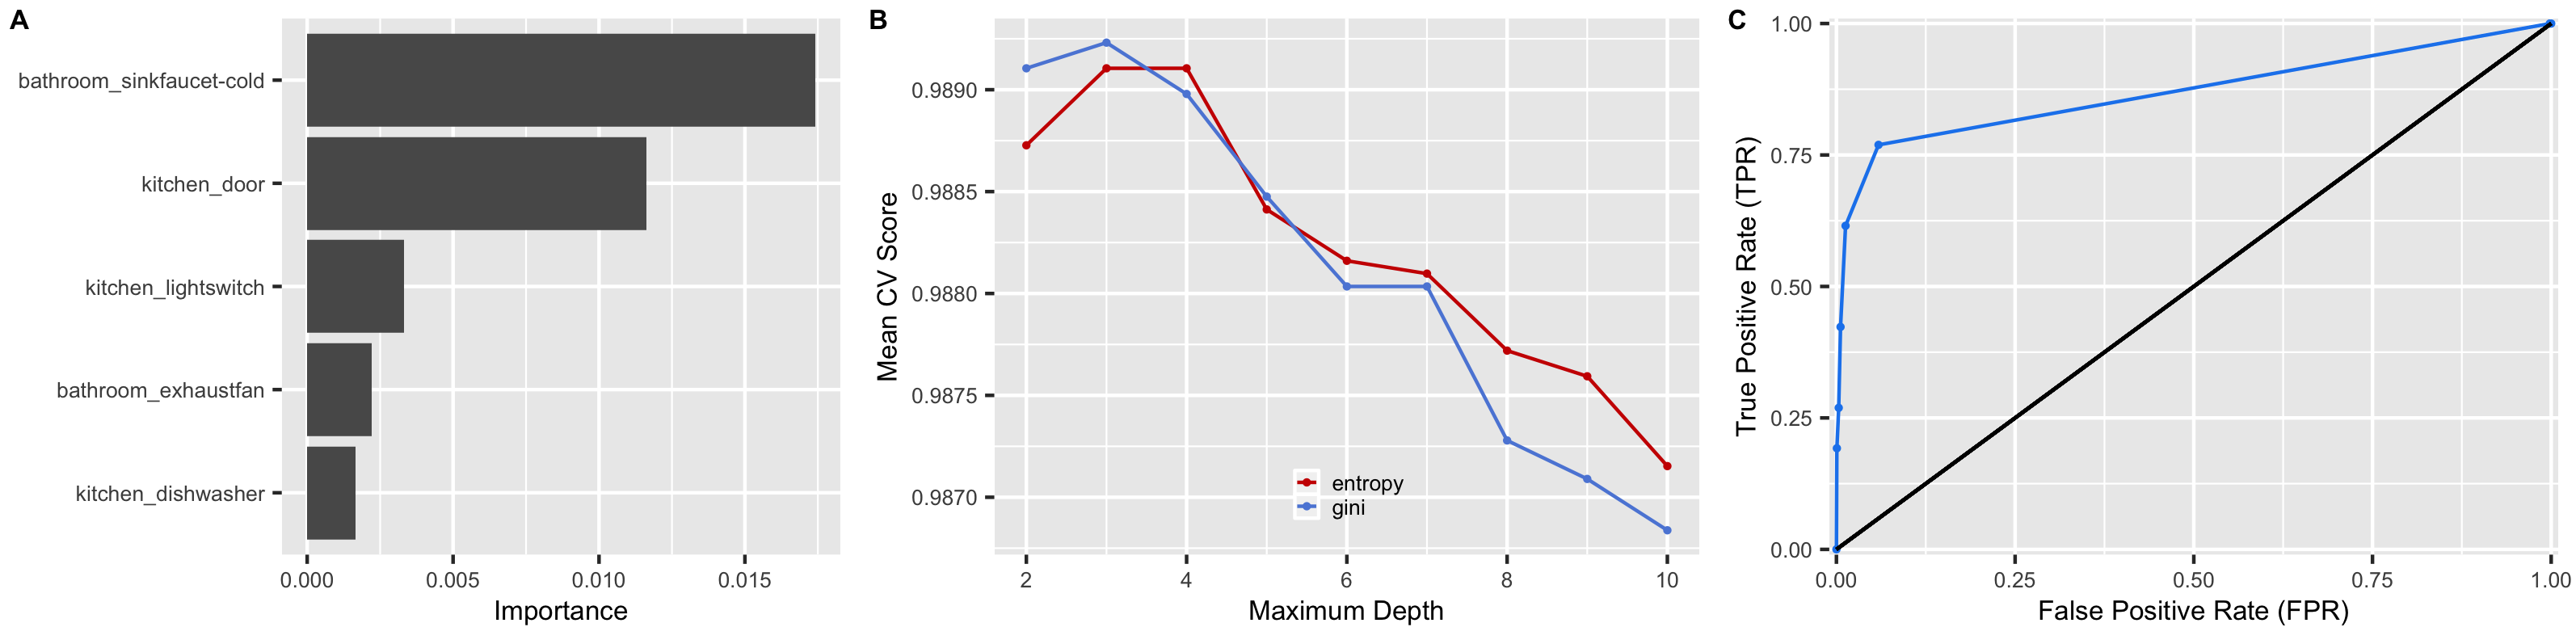
\includegraphics[width=1\linewidth]{/Users/alistairgj/Documents/GitHub/IoT_ResearchProject/IoT_November/images/kitchen_washingmachine_allFeatures} 

}

\caption{ADD TEXT}\label{fig:unnamed-chunk-12}
\end{figure}

\pagebreak

\hypertarget{kitchen-lightswitch}{%
\subsubsection{Kitchen Lightswitch}\label{kitchen-lightswitch}}

\begin{itemize}
\tightlist
\item
  Confusion matrix
\item
  KPIs
\end{itemize}

Fitting 15 folds for each of 18 candidates, totalling 270 fits
\href{Done\%20270\%20out\%20of\%20270\%20\%7C\%20elapsed:\%202.1s\%20finished}{Parallel(n\_jobs=1)}:
Done 270 out of 270 \textbar{} elapsed: 3.4s finished best params:
\{`criterion': `gini', `max\_depth': 10\} best score: 0.797153473140626

\begin{verbatim}
      precision    recall  f1-score   support

     0.0       0.88      0.87      0.87      1100
     1.0       0.71      0.74      0.72       488

accuracy                           0.83      1588
\end{verbatim}

macro avg 0.80 0.80 0.80 1588 weighted avg 0.83 0.83 0.83 1588

{[}{[}952 148{]} {[}127 361{]}{]} Fitting 15 folds for each of 18
candidates, totalling 270 fits
\href{Done\%20270\%20out\%20of\%20270\%20\%7C\%20elapsed:\%202.1s\%20finished}{Parallel(n\_jobs=1)}:
Using backend SequentialBackend with 1 concurrent workers.
\href{Done\%20270\%20out\%20of\%20270\%20\%7C\%20elapsed:\%202.1s\%20finished}{Parallel(n\_jobs=1)}:
Done 270 out of 270 \textbar{} elapsed: 3.4s finished

\begin{figure}[H]

{\centering 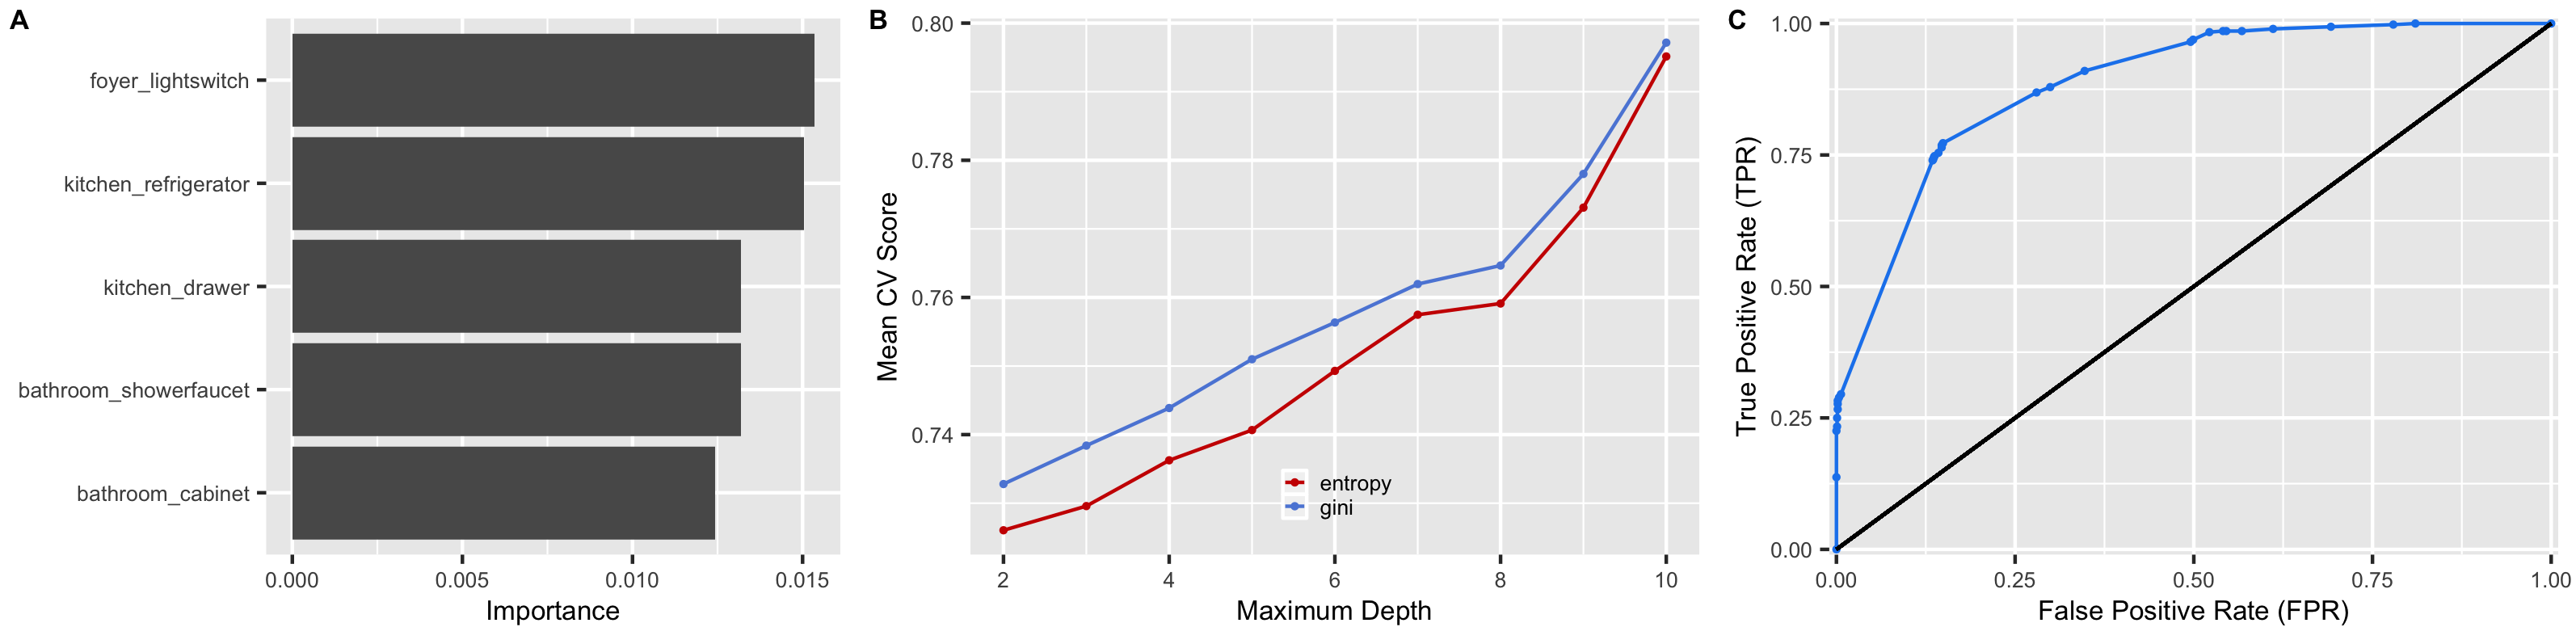
\includegraphics[width=1\linewidth]{/Users/alistairgj/Documents/GitHub/IoT_ResearchProject/IoT_November/images/kitchen_lightswitch_allFeatures} 

}

\caption{ADD TEXT}\label{fig:unnamed-chunk-13}
\end{figure}

\pagebreak

\hypertarget{livingroom-lamp}{%
\subsubsection{Livingroom Lamp}\label{livingroom-lamp}}

\begin{itemize}
\tightlist
\item
  Confusion matrix
\item
  KPIs
\end{itemize}

Fitting 15 folds for each of 18 candidates, totalling 270 fits
\href{Done\%20270\%20out\%20of\%20270\%20\%7C\%20elapsed:\%202.1s\%20finished}{Parallel(n\_jobs=1)}:
Done 270 out of 270 \textbar{} elapsed: 3.4s finished best params:
\{`criterion': `gini', `max\_depth': 8\} best score: 0.8140311102714277

\begin{verbatim}
  precision    recall  f1-score   support

     0.0       0.81      0.99      0.89      1252
     1.0       0.83      0.16      0.27       336

accuracy                           0.82      1588
\end{verbatim}

macro avg 0.82 0.58 0.58 1588 weighted avg 0.82 0.82 0.76 1588

{[}{[}1241 11{]} {[} 282 54{]}{]} Fitting 15 folds for each of 18
candidates, totalling 270 fits
\href{Done\%20270\%20out\%20of\%20270\%20\%7C\%20elapsed:\%202.1s\%20finished}{Parallel(n\_jobs=1)}:
Using backend SequentialBackend with 1 concurrent workers.
\href{Done\%20270\%20out\%20of\%20270\%20\%7C\%20elapsed:\%202.1s\%20finished}{Parallel(n\_jobs=1)}:
Done 270 out of 270 \textbar{} elapsed: 3.0s finished

\begin{figure}[H]

{\centering 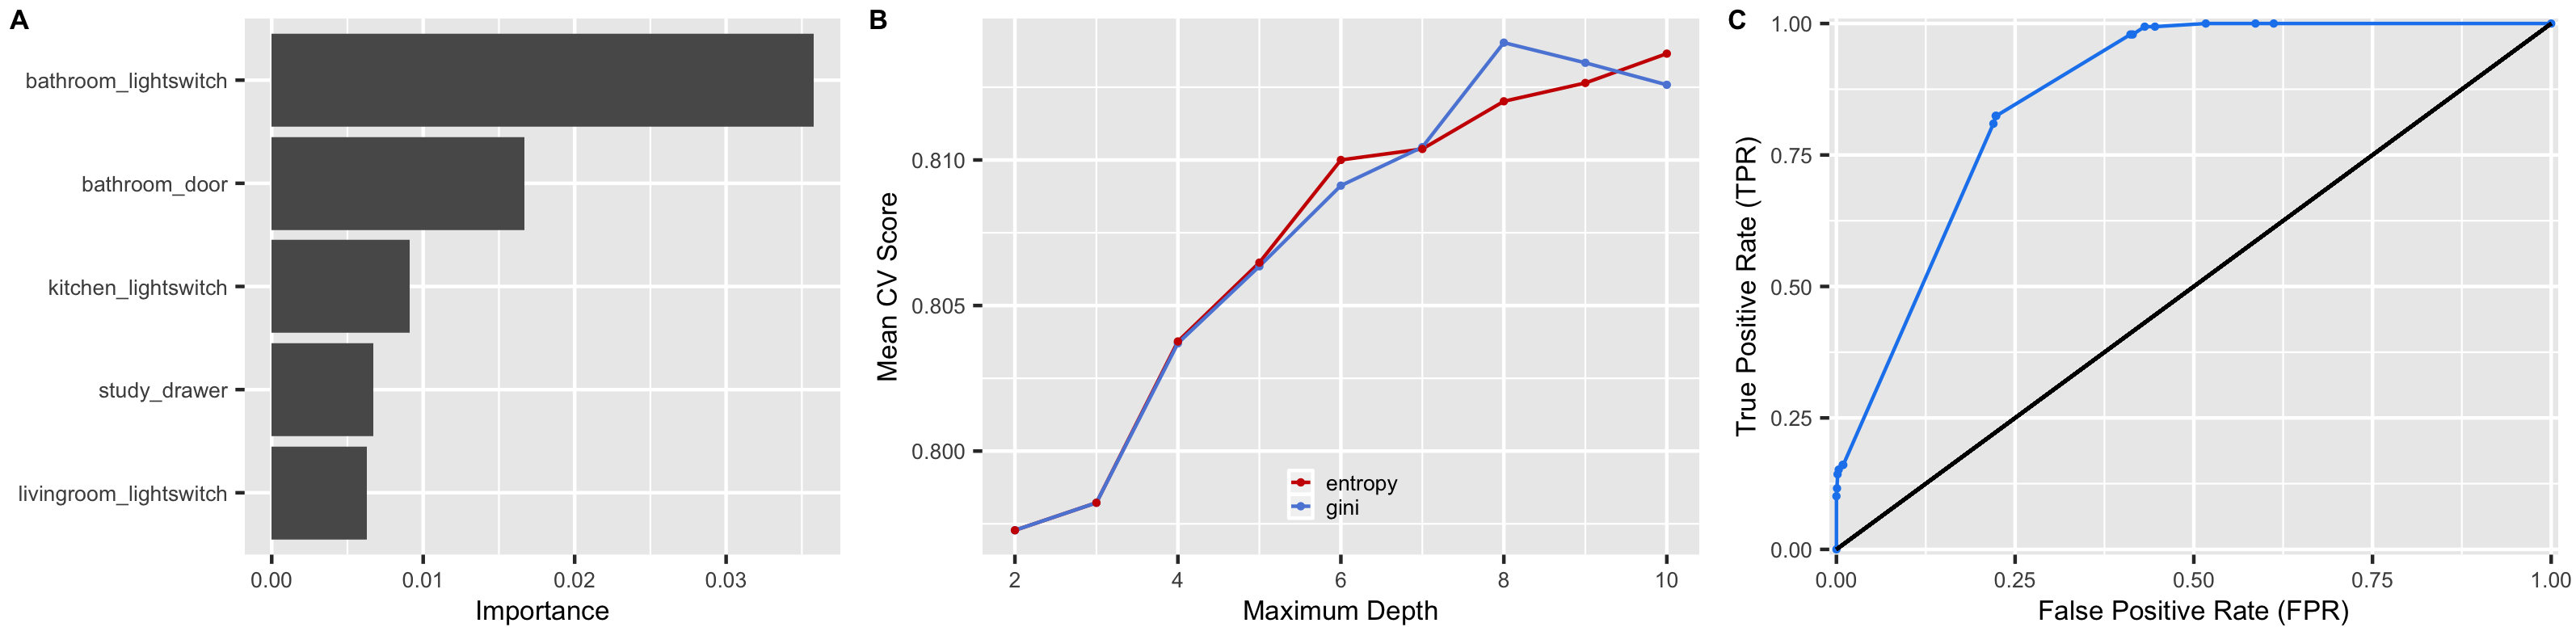
\includegraphics[width=1\linewidth]{/Users/alistairgj/Documents/GitHub/IoT_ResearchProject/IoT_November/images/livingroom_lamp_allFeatures} 

}

\caption{ADD TEXT}\label{fig:unnamed-chunk-14}
\end{figure}

\pagebreak

\hypertarget{kitchen_microwave}{%
\subsubsection{kitchen\_microwave}\label{kitchen_microwave}}

\begin{itemize}
\tightlist
\item
  Confusion matrix
\item
  KPIs
\end{itemize}

Fitting 15 folds for each of 18 candidates, totalling 270 fits
\href{Done\%20270\%20out\%20of\%20270\%20\%7C\%20elapsed:\%202.1s\%20finished}{Parallel(n\_jobs=1)}:
Done 270 out of 270 \textbar{} elapsed: 3.3s finished best params:
\{`criterion': `entropy', `max\_depth': 2\} best score:
0.989042131116569

\begin{verbatim}
 precision    recall  f1-score   support

     0.0       0.99      1.00      1.00      1575
     1.0       0.00      0.00      0.00        13

accuracy                           0.99      1588
\end{verbatim}

macro avg 0.50 0.50 0.50 1588 weighted avg 0.98 0.99 0.99 1588

{[}{[}1575 0{]} {[} 13 0{]}{]} Fitting 15 folds for each of 18
candidates, totalling 270 fits
\href{Done\%20270\%20out\%20of\%20270\%20\%7C\%20elapsed:\%202.1s\%20finished}{Parallel(n\_jobs=1)}:
Using backend SequentialBackend with 1 concurrent workers.
\href{Done\%20270\%20out\%20of\%20270\%20\%7C\%20elapsed:\%202.1s\%20finished}{Parallel(n\_jobs=1)}:
Done 270 out of 270 \textbar{} elapsed: 3.5s finished

\begin{figure}[H]

{\centering 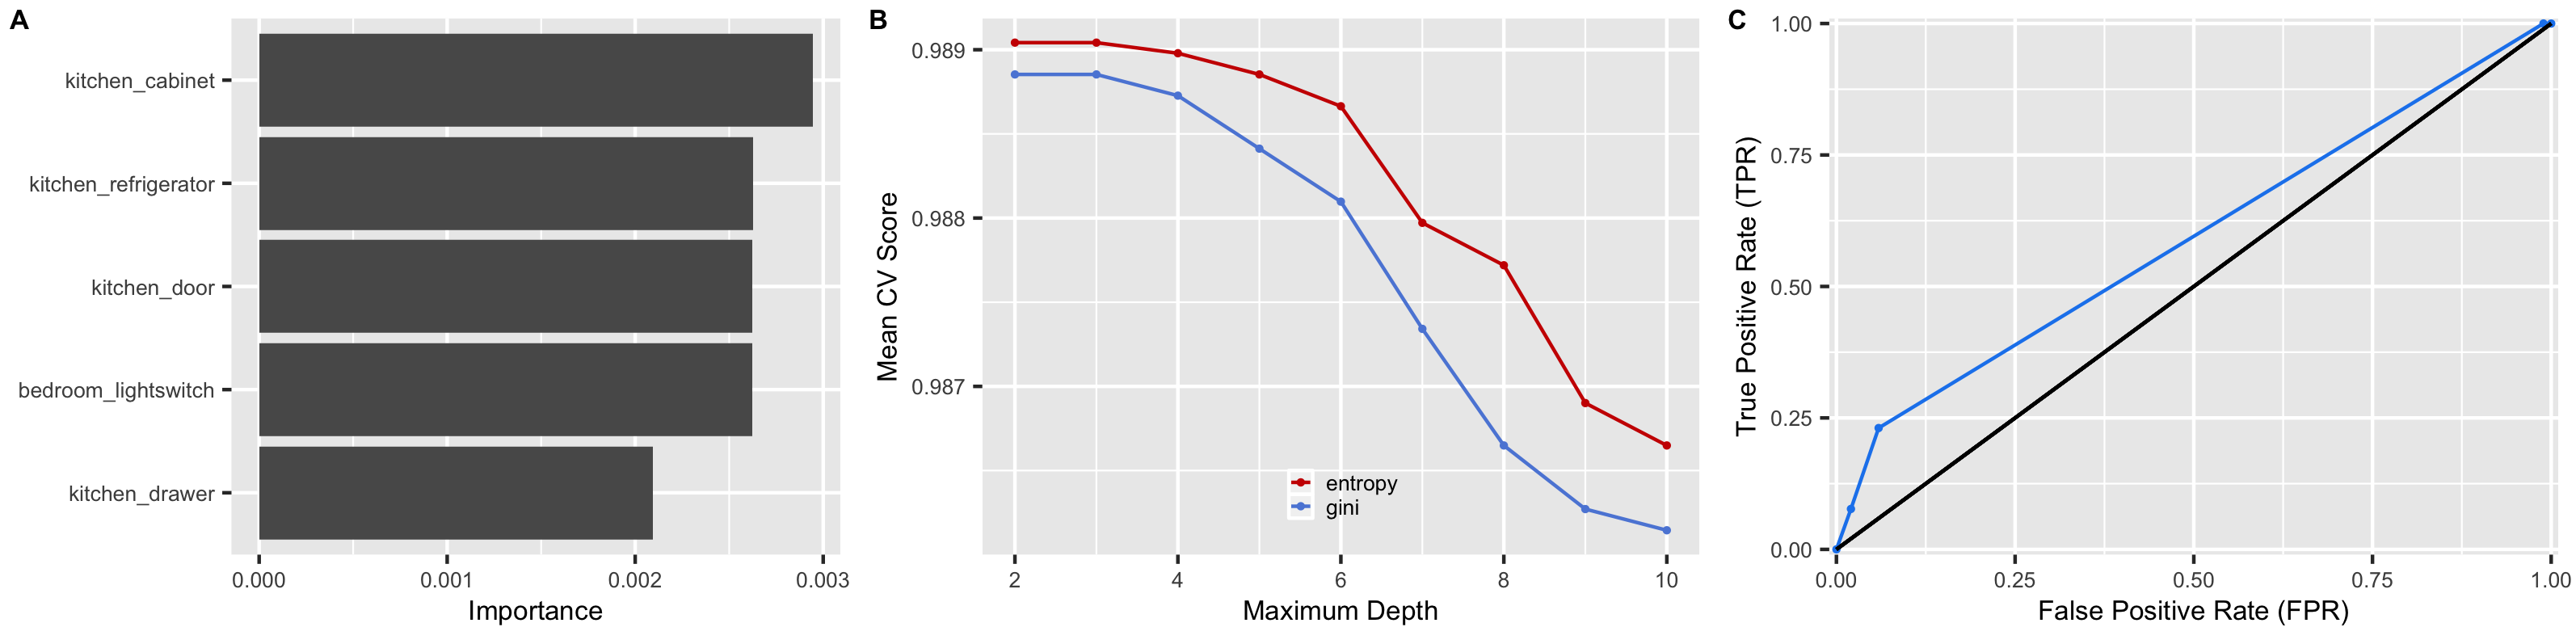
\includegraphics[width=1\linewidth]{/Users/alistairgj/Documents/GitHub/IoT_ResearchProject/IoT_November/images/kitchen_microwave_allFeatures} 

}

\caption{ADD TEXT}\label{fig:unnamed-chunk-15}
\end{figure}

\pagebreak

\hypertarget{kitchen_garbagedisposal}{%
\subsubsection{kitchen\_garbagedisposal}\label{kitchen_garbagedisposal}}

\begin{itemize}
\tightlist
\item
  Confusion matrix
\item
  KPIs
\end{itemize}

Fitting 15 folds for each of 18 candidates, totalling 270 fits
\href{Done\%20270\%20out\%20of\%20270\%20\%7C\%20elapsed:\%202.1s\%20finished}{Parallel(n\_jobs=1)}:
Done 270 out of 270 \textbar{} elapsed: 3.4s finished best params:
\{`criterion': `gini', `max\_depth': 2\} best score: 0.9975439259399207

\begin{verbatim}
   precision    recall  f1-score   support

     0.0       1.00      1.00      1.00      1586
     1.0       0.00      0.00      0.00         2

accuracy                           1.00      1588
\end{verbatim}

macro avg 0.50 0.50 0.50 1588 weighted avg 1.00 1.00 1.00 1588

{[}{[}1586 0{]} {[} 2 0{]}{]} Fitting 15 folds for each of 18
candidates, totalling 270 fits
\href{Done\%20270\%20out\%20of\%20270\%20\%7C\%20elapsed:\%202.1s\%20finished}{Parallel(n\_jobs=1)}:
Using backend SequentialBackend with 1 concurrent workers.
\href{Done\%20270\%20out\%20of\%20270\%20\%7C\%20elapsed:\%202.1s\%20finished}{Parallel(n\_jobs=1)}:
Done 270 out of 270 \textbar{} elapsed: 2.9s finished

\begin{figure}[H]

{\centering 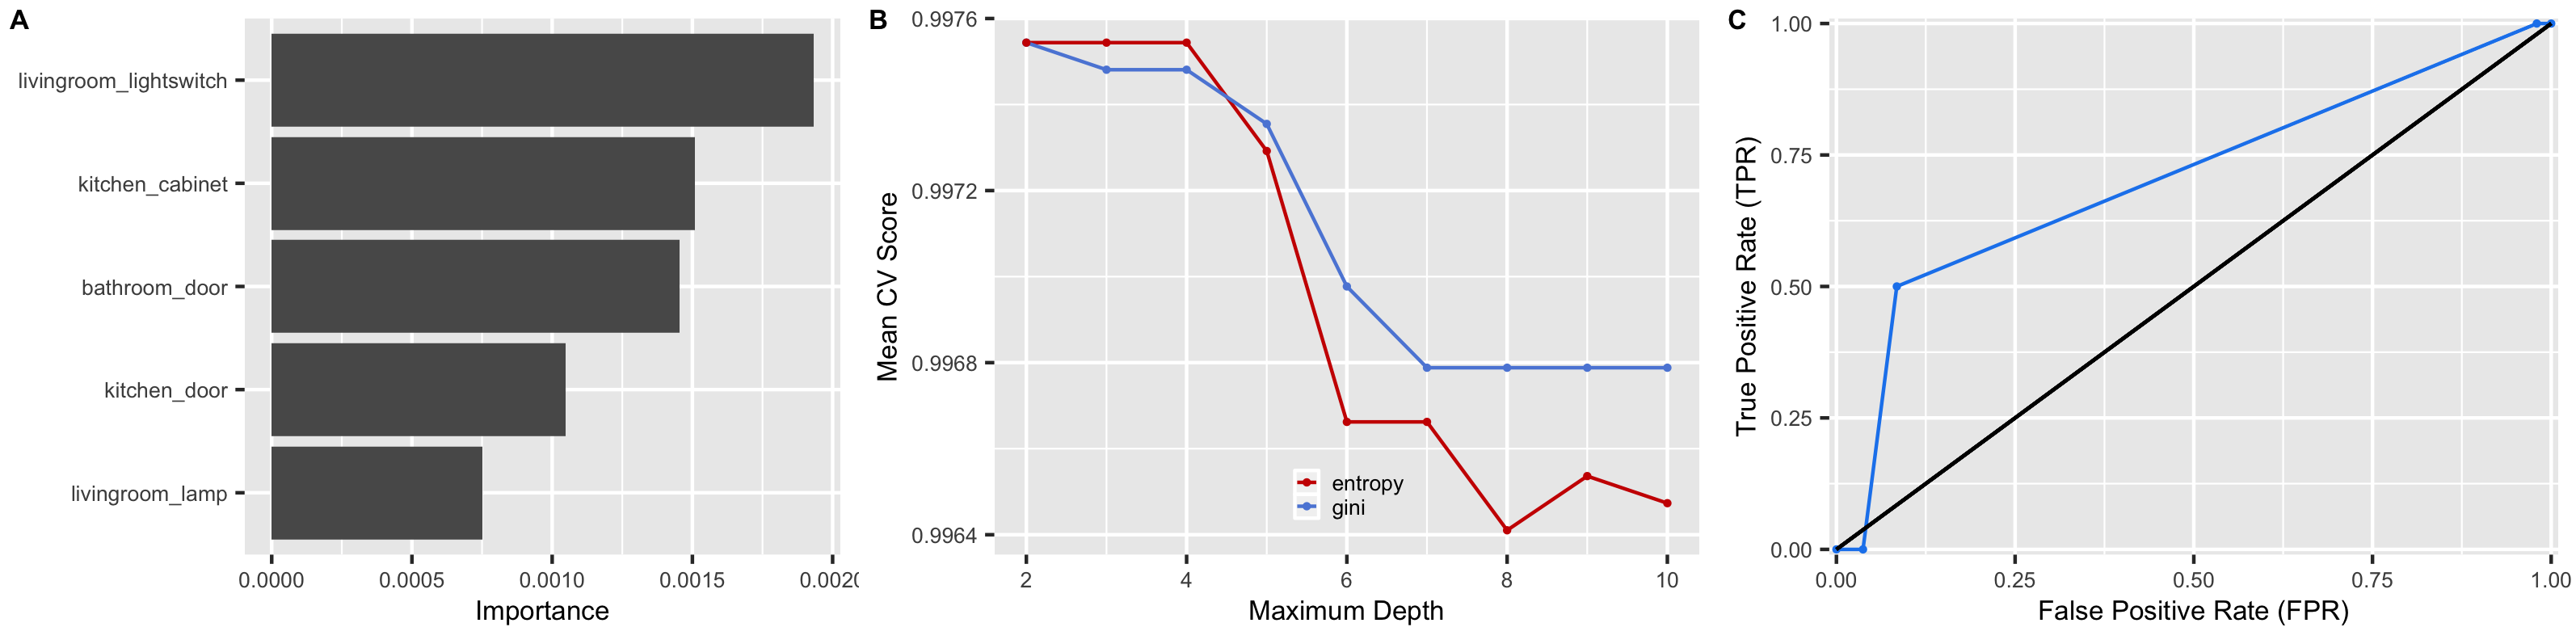
\includegraphics[width=1\linewidth]{/Users/alistairgj/Documents/GitHub/IoT_ResearchProject/IoT_November/images/kitchen_garbagedisposal_allFeatures} 

}

\caption{ADD TEXT}\label{fig:unnamed-chunk-16}
\end{figure}

\pagebreak

\hypertarget{kitchen_coffeemachine}{%
\subsubsection{kitchen\_coffeemachine}\label{kitchen_coffeemachine}}

\begin{itemize}
\tightlist
\item
  Confusion matrix
\item
  KPIs
\end{itemize}

Fitting 15 folds for each of 18 candidates, totalling 270 fits
\href{Done\%20270\%20out\%20of\%20270\%20\%7C\%20elapsed:\%202.1s\%20finished}{Parallel(n\_jobs=1)}:
Done 270 out of 270 \textbar{} elapsed: 3.2s finished best params:
\{`criterion': `gini', `max\_depth': 2\} best score: 0.9986774985830342

\begin{verbatim}
   precision    recall  f1-score   support

     0.0       1.00      1.00      1.00      1587
     1.0       0.00      0.00      0.00         1

accuracy                           1.00      1588
\end{verbatim}

macro avg 0.50 0.50 0.50 1588 weighted avg 1.00 1.00 1.00 1588

{[}{[}1587 0{]} {[} 1 0{]}{]} Fitting 15 folds for each of 18
candidates, totalling 270 fits
\href{Done\%20270\%20out\%20of\%20270\%20\%7C\%20elapsed:\%202.1s\%20finished}{Parallel(n\_jobs=1)}:
Using backend SequentialBackend with 1 concurrent workers.
\href{Done\%20270\%20out\%20of\%20270\%20\%7C\%20elapsed:\%202.1s\%20finished}{Parallel(n\_jobs=1)}:
Done 270 out of 270 \textbar{} elapsed: 3.1s finished

\begin{figure}[H]

{\centering 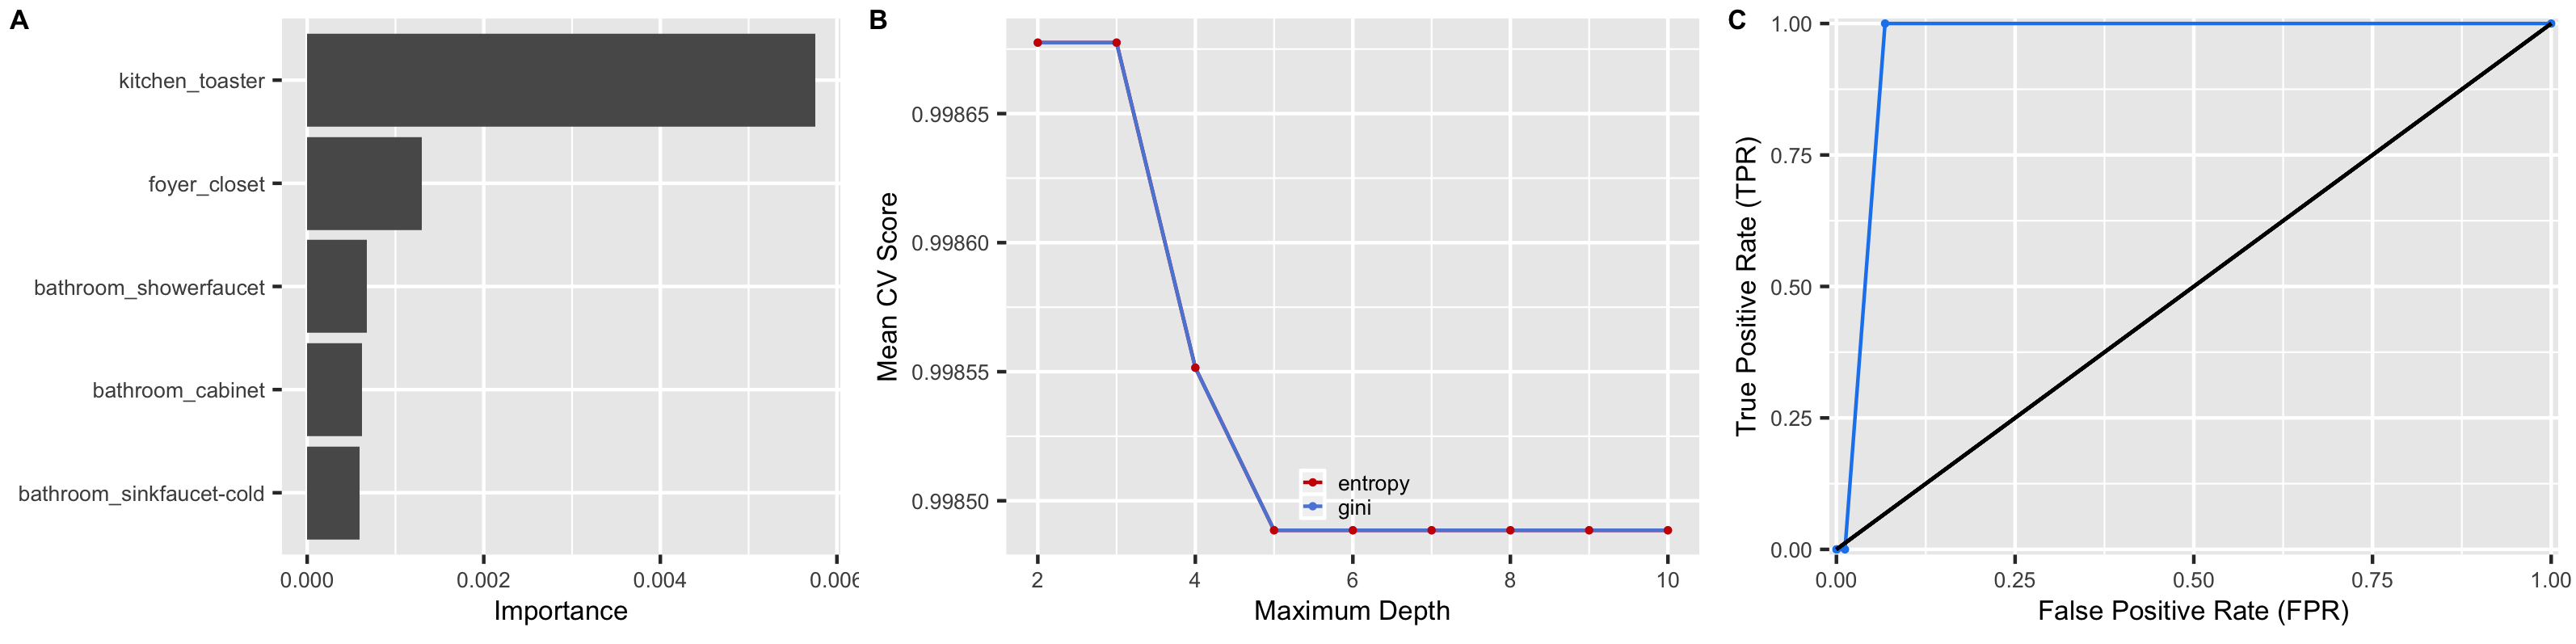
\includegraphics[width=1\linewidth]{/Users/alistairgj/Documents/GitHub/IoT_ResearchProject/IoT_November/images/kitchen_coffeemachine_allFeatures} 

}

\caption{ADD TEXT}\label{fig:unnamed-chunk-17}
\end{figure}

\pagebreak

\hypertarget{livingroom_lightswitch}{%
\subsubsection{livingroom\_lightswitch}\label{livingroom_lightswitch}}

\begin{itemize}
\tightlist
\item
  Confusion matrix
\item
  KPIs
\end{itemize}

Fitting 15 folds for each of 18 candidates, totalling 270 fits
\href{Done\%20270\%20out\%20of\%20270\%20\%7C\%20elapsed:\%202.1s\%20finished}{Parallel(n\_jobs=1)}:
Done 270 out of 270 \textbar{} elapsed: 3.6s finished best params:
\{`criterion': `entropy', `max\_depth': 7\} best score:
0.9080546633919012

\begin{verbatim}
     precision    recall  f1-score   support

     0.0       0.91      1.00      0.95      1386
     1.0       1.00      0.28      0.44       202

accuracy                           0.91      1588
\end{verbatim}

macro avg 0.95 0.64 0.70 1588 weighted avg 0.92 0.91 0.89 1588

{[}{[}1386 0{]} {[} 145 57{]}{]} Fitting 15 folds for each of 18
candidates, totalling 270 fits
\href{Done\%20270\%20out\%20of\%20270\%20\%7C\%20elapsed:\%202.1s\%20finished}{Parallel(n\_jobs=1)}:
Using backend SequentialBackend with 1 concurrent workers.
\href{Done\%20270\%20out\%20of\%20270\%20\%7C\%20elapsed:\%202.1s\%20finished}{Parallel(n\_jobs=1)}:
Done 270 out of 270 \textbar{} elapsed: 4.0s finished

\begin{figure}[H]

{\centering 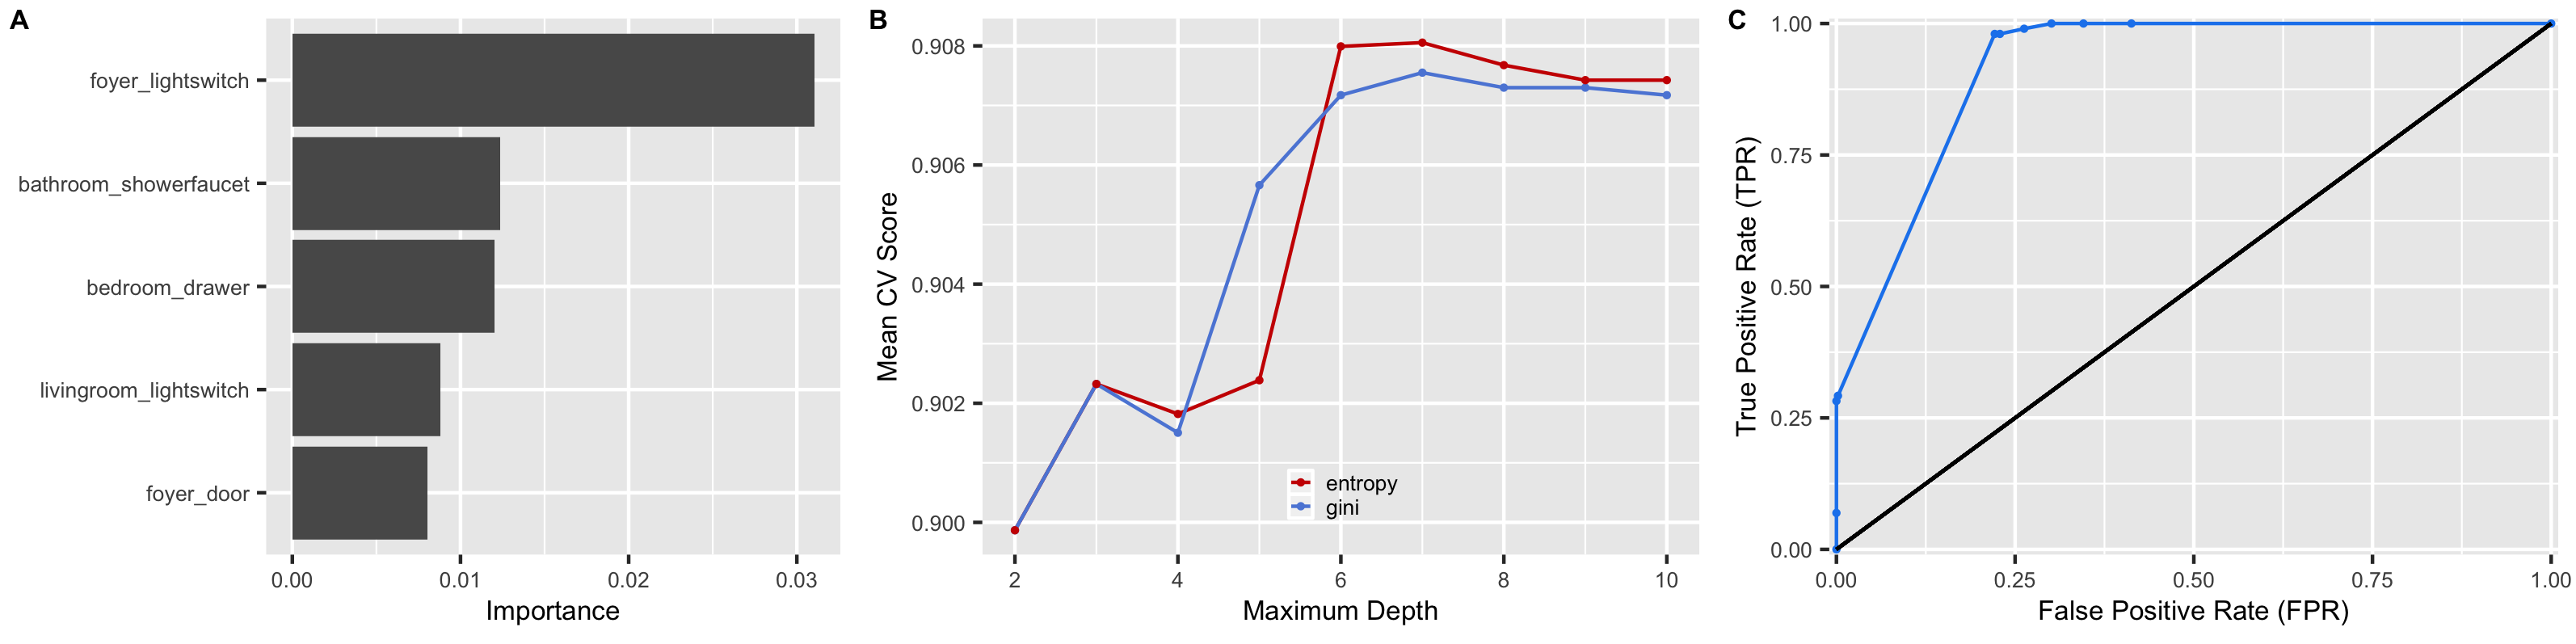
\includegraphics[width=1\linewidth]{/Users/alistairgj/Documents/GitHub/IoT_ResearchProject/IoT_November/images/livingroom_lightswitch_allFeatures} 

}

\caption{ADD TEXT}\label{fig:unnamed-chunk-18}
\end{figure}

\pagebreak

\hypertarget{kitchen_oven}{%
\subsubsection{kitchen\_oven}\label{kitchen_oven}}

\begin{itemize}
\tightlist
\item
  Confusion matrix
\item
  KPIs
\end{itemize}

Fitting 15 folds for each of 18 candidates, totalling 270 fits
\href{Done\%20270\%20out\%20of\%20270\%20\%7C\%20elapsed:\%202.1s\%20finished}{Parallel(n\_jobs=1)}:
Done 270 out of 270 \textbar{} elapsed: 3.3s finished best params:
\{`criterion': `entropy', `max\_depth': 2\} best score:
0.9951508281377921

\begin{verbatim}
   precision    recall  f1-score   support

     0.0       0.99      1.00      1.00      1579
     1.0       0.00      0.00      0.00         9

accuracy                           0.99      1588
\end{verbatim}

macro avg 0.50 0.50 0.50 1588 weighted avg 0.99 0.99 0.99 1588

{[}{[}1579 0{]} {[} 9 0{]}{]} Fitting 15 folds for each of 18
candidates, totalling 270 fits
\href{Done\%20270\%20out\%20of\%20270\%20\%7C\%20elapsed:\%202.1s\%20finished}{Parallel(n\_jobs=1)}:
Using backend SequentialBackend with 1 concurrent workers.
\href{Done\%20270\%20out\%20of\%20270\%20\%7C\%20elapsed:\%202.1s\%20finished}{Parallel(n\_jobs=1)}:
Done 270 out of 270 \textbar{} elapsed: 3.4s finished

\begin{figure}[H]

{\centering 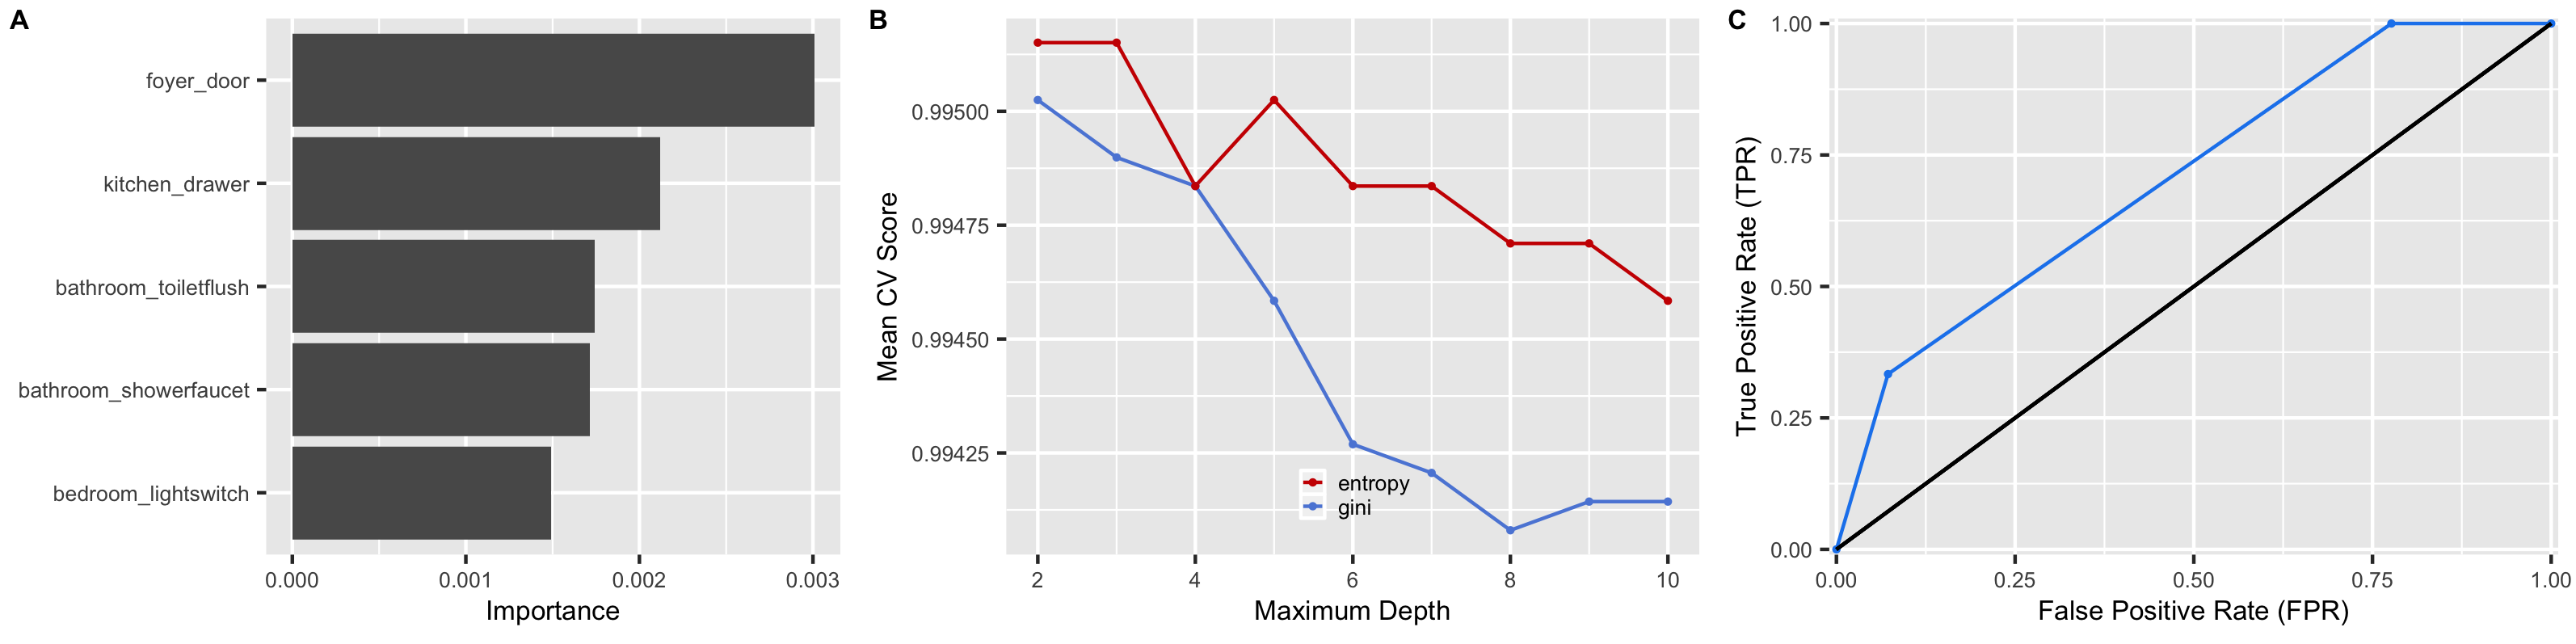
\includegraphics[width=1\linewidth]{/Users/alistairgj/Documents/GitHub/IoT_ResearchProject/IoT_November/images/kitchen_oven_allFeatures} 

}

\caption{ADD TEXT}\label{fig:unnamed-chunk-19}
\end{figure}

\pagebreak

\hypertarget{kitchen_dishwasher}{%
\subsubsection{kitchen\_dishwasher}\label{kitchen_dishwasher}}

\begin{itemize}
\tightlist
\item
  Confusion matrix
\item
  KPIs
\end{itemize}

Fitting 15 folds for each of 18 candidates, totalling 270 fits
\href{Done\%20270\%20out\%20of\%20270\%20\%7C\%20elapsed:\%202.1s\%20finished}{Parallel(n\_jobs=1)}:
Done 270 out of 270 \textbar{} elapsed: 3.8s finished best params:
\{`criterion': `entropy', `max\_depth': 8\} best score:
0.949870898671201

\begin{verbatim}
       precision    recall  f1-score   support

     0.0       0.96      0.99      0.98      1496
     1.0       0.75      0.26      0.39        92

accuracy                           0.95      1588
\end{verbatim}

macro avg 0.85 0.63 0.68 1588 weighted avg 0.94 0.95 0.94 1588

{[}{[}1488 8{]} {[} 68 24{]}{]} Fitting 15 folds for each of 18
candidates, totalling 270 fits
\href{Done\%20270\%20out\%20of\%20270\%20\%7C\%20elapsed:\%202.1s\%20finished}{Parallel(n\_jobs=1)}:
Using backend SequentialBackend with 1 concurrent workers.
\href{Done\%20270\%20out\%20of\%20270\%20\%7C\%20elapsed:\%202.1s\%20finished}{Parallel(n\_jobs=1)}:
Done 270 out of 270 \textbar{} elapsed: 4.0s finished

\begin{figure}[H]

{\centering 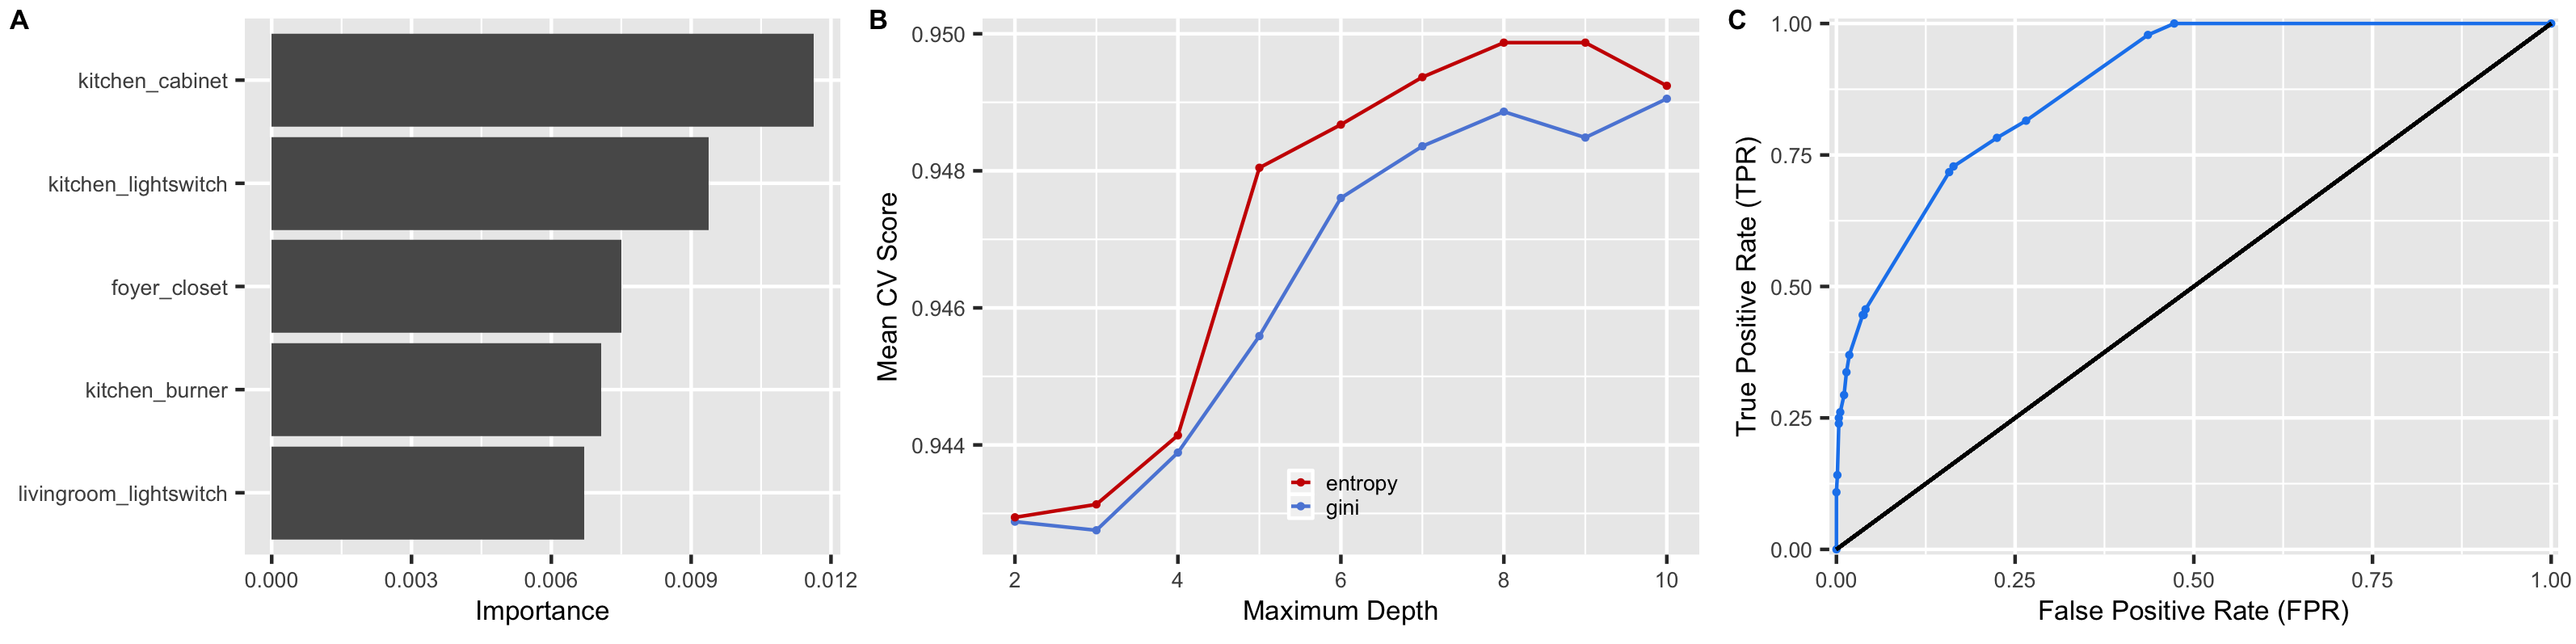
\includegraphics[width=1\linewidth]{/Users/alistairgj/Documents/GitHub/IoT_ResearchProject/IoT_November/images/kitchen_dishwasher_allFeatures} 

}

\caption{ADD TEXT}\label{fig:unnamed-chunk-20}
\end{figure}

\pagebreak

\hypertarget{bathroom_sinkfaucet-hot}{%
\subsubsection{bathroom\_sinkfaucet-hot}\label{bathroom_sinkfaucet-hot}}

\begin{itemize}
\tightlist
\item
  Confusion matrix
\item
  KPIs
\end{itemize}

Fitting 15 folds for each of 18 candidates, totalling 270 fits
\href{Done\%20270\%20out\%20of\%20270\%20\%7C\%20elapsed:\%202.1s\%20finished}{Parallel(n\_jobs=1)}:
Done 270 out of 270 \textbar{} elapsed: 5.6s finished best params:
\{`criterion': `entropy', `max\_depth': 6\} best score:
0.9702752062472448

\begin{verbatim}
  precision    recall  f1-score   support

     0.0       0.97      1.00      0.98      1514
     1.0       0.86      0.42      0.56        74

accuracy                           0.97      1588
\end{verbatim}

macro avg 0.92 0.71 0.77 1588 weighted avg 0.97 0.97 0.96 1588

{[}{[}1509 5{]} {[} 43 31{]}{]} Fitting 15 folds for each of 18
candidates, totalling 270 fits
\href{Done\%20270\%20out\%20of\%20270\%20\%7C\%20elapsed:\%202.1s\%20finished}{Parallel(n\_jobs=1)}:
Using backend SequentialBackend with 1 concurrent workers.
\href{Done\%20270\%20out\%20of\%20270\%20\%7C\%20elapsed:\%202.1s\%20finished}{Parallel(n\_jobs=1)}:
Done 270 out of 270 \textbar{} elapsed: 3.5s finished

\begin{figure}[H]

{\centering 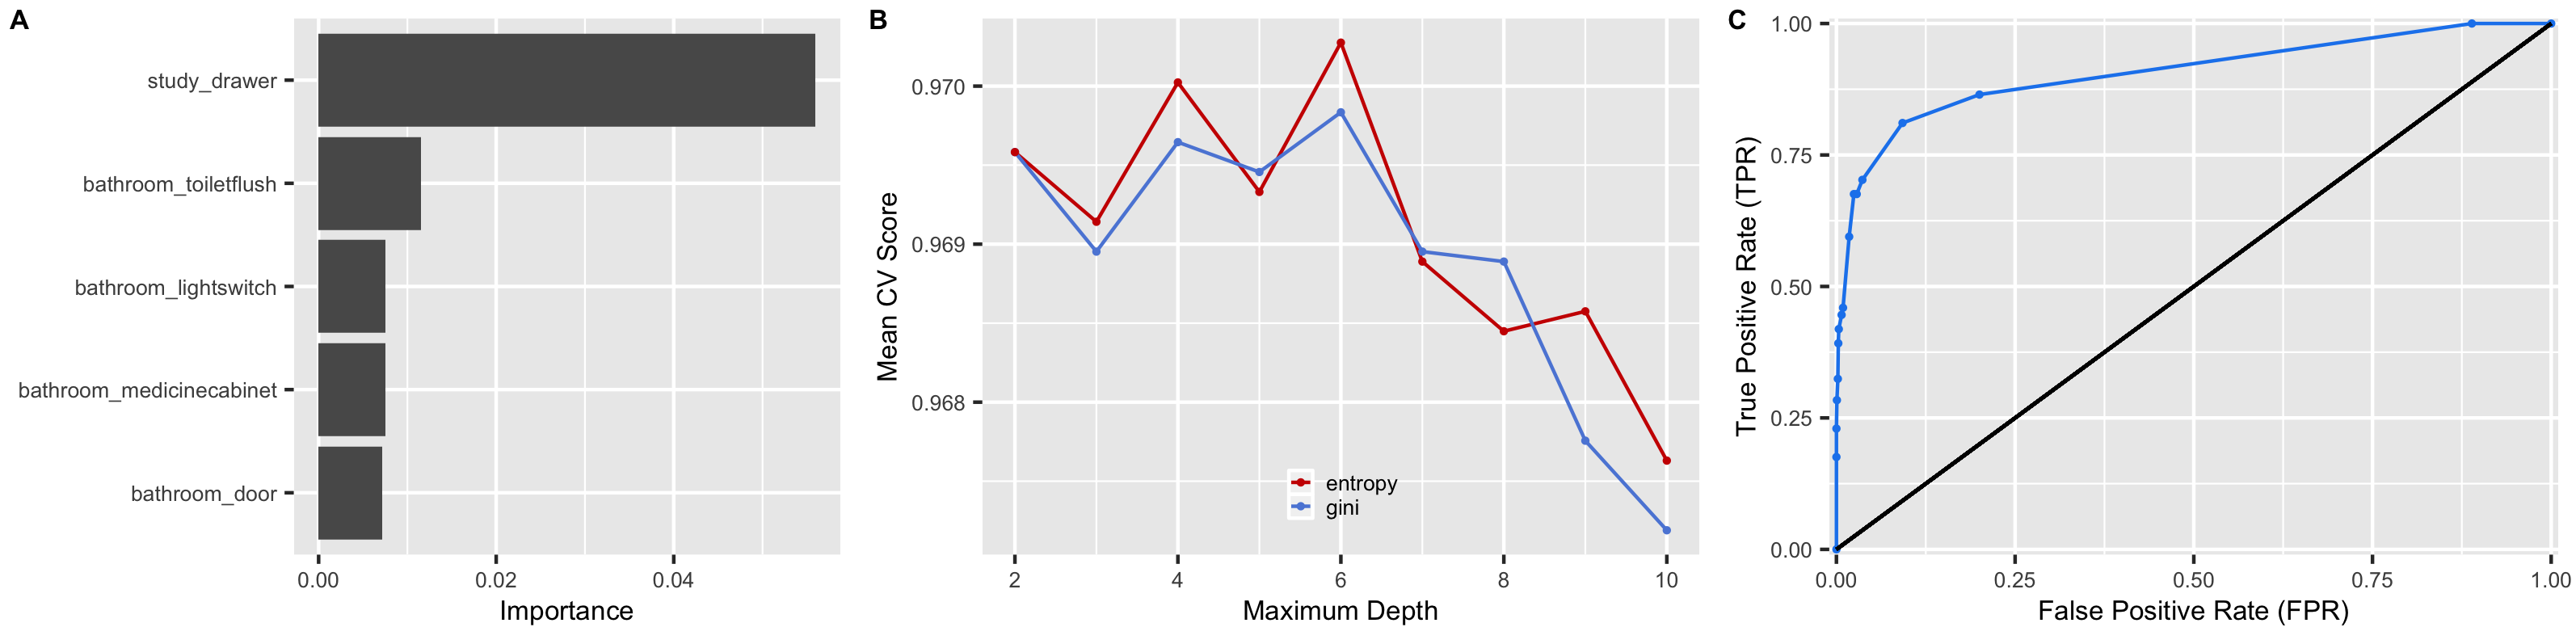
\includegraphics[width=1\linewidth]{/Users/alistairgj/Documents/GitHub/IoT_ResearchProject/IoT_November/images/bathroom_sinkfaucet-hot_allFeatures} 

}

\caption{ADD TEXT}\label{fig:unnamed-chunk-21}
\end{figure}

\hypertarget{references}{%
\section{References}\label{references}}


\end{document}
